\section{Numerical Experiments}
\label{sec:empirical-validation}

This section presents numerical experiments on the reflected noisy cubic control system of Section~\ref{sec:duffing-example}. These experiments illustrate our analytical results and explore how the self-consistent transfer operator framework performs in realistic control regimes beyond our formal hypotheses.

Section~\ref{sec:numerical-implementation} summarizes the numerical implementation of the coupled dynamics. We contrast the exact distributional operator $\Phi_\delta$ (discretized on an Ulam grid) with finite-sample particle simulations ($N<\infty$) driven by a one-step tracking-error gradient estimator. We quantify two effects introduced by finite-sample online learning: boundary reflection bias on the Gaussian tails and the $O(\sigma\sqrt{\delta/N})$ stochastic fluctuation floor. The subsequent experiments fall into two parts:

\begin{itemize}
    \item \emph{Quantitative verification of the local theory (Section~\ref{sec:part1-illustration}):} In the autonomous adaptation protocol, $(\mu_n,\theta_n)$ jointly evolve under $\Phi_\delta$ from $(\mu_0,\theta_0)$ at $\sigma=0.18$. These experiments test the predictions of Sections~\ref{5}--\ref{sec:duffing-example}: existence and the $O(\lambda)$ equilibrium shift under small regularization (Propositions~\ref{prop:duffing-constructive-existence} and~\ref{prop:duffing-small-regularization}), local exponential stability for small learning rates (Theorem~\ref{thm:local-stability}), the exact statistical linear-response contribution $C_*R_*B_*$ to the effective Jacobian $\mathcal J_* = D\overline G(\theta_*)$ (Proposition~\ref{prop:effective-jacobian-identification}), and the slow relaxation rates
    \[
      \lambda_j^{\rm slow}(\delta)
      =
      1-\delta\lambda_j\!\left(
        \Gammahat D\overline G(\theta_*)
      \right)+o(\delta),
    \]
    which yield an asymptotic relaxation time of order $\delta^{-1}$.
    \item \emph{Extension to realistic engineering regimes (Sections~\ref{sec:part2-practice} and~\ref{sec:nonconvex_extension}):} In practical robotic and control applications \cite{lippi2018prediction,lippi2021icinco,DulacArnoldEtAl2021,BrunkeEtAl2022}, controllers are often pre-trained offline under conservative conditions. They are then deployed online under finite time horizons, weak persistent excitation \cite{AnnaswamyFradkov2021,VernadeEtAl2026}, non-infinitesimal learning rates, or nonlinear network architectures. Section~\ref{sec:part2-practice} investigates these effects. It includes a two-phase deployment protocol where a parameter $\theta_{\rm off}$ identified under a conservative baseline gain ($-0.80$) is released online under a relaxed gain ($-0.25$) \cite{LippiActionError}. Section~\ref{sec:nonconvex_extension} explores a multilayer perceptron compensator. In the unregularized, exactly realizable case with $\Gammahat=\Id$, $C_*=0$, and parameter multipliers $1-\delta\lambda_j(H_*)$, we test how far the learning rate can be pushed across and beyond the linear stability threshold
    \[
      \delta_c=\frac{2}{\lambda_{\max}(H_*)}.
    \]
\end{itemize}

Figure~\ref{fig:block_diagram} shows the control architecture.

\begin{figure}[htpb]
\centering
\begin{tikzpicture}[
    auto,
    block/.style={rectangle, draw, thick, align=center, minimum height=1.2cm},
    sum/.style={circle, draw, thick, inner sep=0pt, minimum size=6mm},
    line/.style={draw, thick, -{Stealth[length=2.5mm]}},
    optional/.style={rectangle, draw, thick, dashed, align=center, minimum height=1.2cm, fill=white}
]

% Main Sum (u_n)
\node [sum] (sum_u) at (0,0) {$\Sigma$};

% Cubic Plant Dynamics
\node [block] (duffing) at (3.5, 0) {\textbf{Cubic Plant Dynamics} \\ $1.05x_n + 0.15x_n^3 + u_n$};

% Noise Sum
\node [sum] (sum_noise) at (6.8, 0) {$\Sigma$};

% Reflection
\node [block] (reflect) at (9.5, 0) {\textbf{Reflection} \\ $\mathfrak{r}_2(\cdot)$};

% Output
\node (output) at (13, 0) {};

% Noises
\node [align=center] (proc_noise) at (6.8, 1.8) {Process \\ Noise $\xi_n$};

% Plant box
\begin{scope}[on background layer]
    \node [draw=black!70, thick, dashed, fill=green!5, inner sep=4mm, fit=(duffing) (sum_noise) (reflect), label={[font=\bfseries, yshift=-1mm]below:Physical Plant}] (plant_box) {};
\end{scope}

% Controllers
\node [block] (baseline) at (5, -2.5) {\textbf{Baseline Controller} \\ $u_{\rm base}(x_n) = -0.25x_n$};
\node [optional] (nn) at (5, -4.5) {\textbf{Neural Compensator} \\ $g(x_n, \theta_n)$ \\ {\footnotesize (Polynomial or MLP)}};

% Connections
\draw [line] (sum_u) -- node [above] {$u_n$} (duffing);
\draw [line] (duffing) -- (sum_noise);
\draw [line] (proc_noise) -- (sum_noise);
\draw [line] (sum_noise) -- (reflect);
\draw [thick] (reflect) -- (12,0) coordinate (y_coord);
\draw [line] (12,0) -- node [above] {$x_n$} (output);

% Feedback paths
\draw [thick] (y_coord) |- (baseline.east);
\draw [line] (y_coord) |- (nn.east);

\draw [line] (baseline.west) -| node[pos=0.9, right] {$+$} (sum_u.south);
\draw [line] (nn.west) -- (-1.5, -4.5) |- node[pos=0.9, above] {$-$} (sum_u.west);

\end{tikzpicture}
\caption{Block diagram of the closed-loop system. The plant has cubic drift $1.05x_n + 0.15x_n^3$, stabilized locally around $x_{\rm ref}=0$ by $u_{\rm base}(x_n) = -0.25x_n$, perturbed by $\xi_n \sim \mathcal{N}(0,\sigma^2)$, and folded onto $X=[-2,2]$ by $\mathfrak{r}_2(\cdot)$. In Part~1 (Figures~\ref{fig:part1_nominal_convergence} and~\ref{fig:part1_timescale_and_reg}), $\sigma=0.18$. In Part~2, $\sigma$ is reduced to $0.10$ and $0.05$ to study the invariance residual $\mathfrak{R}_A$, ill-conditioning of the Gram matrix, and loss of linear stability. The compensator $g(x_n,\theta_n)$ acts with opposite sign to cancel $d(x_n)$ and is parameterized by a polynomial basis (Figures~\ref{fig:part1_nominal_convergence}--\ref{fig:part2_density_shattering}) or a multilayer perceptron (Figure~\ref{fig:mlp_convergence}).}
\label{fig:block_diagram}
\end{figure}

\subsection{Numerical Implementation}
\label{sec:numerical-implementation}

Recall the reflected stochastic plant of Section~\ref{sec:duffing-example}, the baseline controller $u_{\rm base}(x) = -0.25x$, and the target cubic residual $d(x) = 0.15x^3$. We assume Gaussian process noise $\xi_n \sim \mathcal{N}(0,\sigma^2)$.

The bound $\norm{d}_{L^\infty(X)} = 1.2$ on $X=[-2,2]$ sets the existence radius $r_{\rm ex} = (\norm{\theta_c}S_\psi + 1.2)S_\psi/\lambda$ used in Proposition~\ref{prop:duffing-constructive-existence}. We evaluate the neural compensator $g(x,\theta) = \theta^{\mathsf T}\psi(x)$ using the polynomial feature map
\begin{equation}
    \psi(x) = [1, x, x^2, x^3]^{\mathsf T}.
\end{equation}
Since $\psi(x)$ spans $d(x)$, the unique parameter satisfying $g(\cdot,\theta_{\rm opt}) \equiv d(\cdot)$ is
\begin{equation}
    \theta_{\rm opt} = [0, 0, 0, 0.15]^{\mathsf T}.
\end{equation}
Reflection symmetry of $\mu_{\theta_{\rm opt}}$ decouples the unregularized Gram matrix $H_* = Q_{\rm opt} = \int_X \psi\psi^{\mathsf T}\dd\mu_{\theta_{\rm opt}}$ into even and odd blocks, where the odd block is
\[
  H_{\rm odd} = \begin{pmatrix} m_2 & m_4 \\ m_4 & m_6 \end{pmatrix}, \qquad m_{2k} = \int_X x^{2k}\dd\mu_{\theta_{\rm opt}}(x).
\]
Approximating $\mu_{\theta_{\rm opt}}$ by the unreflected stationary Gaussian law of variance $\sigma_x^2 = \sigma^2/0.36$ gives $\det(H_{\rm odd}) = 6\sigma_x^8$ and
\begin{equation}
    \lambda_{\min}(H_*) \approx 6\sigma_x^6 \approx 128.6\,\sigma^6.
    \label{eq:duffing-sigma6-law}
\end{equation}
This estimate yields $\lambda_{\min}(H_*) \approx 4.37\times 10^{-3}$ at $\sigma=0.18$ (Section~\ref{sec:part1-illustration}) and $\lambda_{\min}(H_*) \approx 1.29\times 10^{-4}$ at $\sigma=0.10$ (Section~\ref{sec:part2-practice}).

To approximate the uniform convergence bound \eqref{eq:duffing-controller-convergence}, we evaluate the following quantity on a uniform grid of $K=500$ points $\{x_k\}_{k=1}^K \subset [-2, 2]$:
\begin{equation}
    \mathcal{E}_\infty^{\rm grid}(\theta_n) := \sqrt{\frac{1}{K}\sum_{k=1}^K \bigl|g(x_k, \theta_n) - g(x_k, \theta_{\rm opt})\bigr|^2}.
\end{equation}
Setting $\widehat H_K:=\frac{1}{K}\sum_{k=1}^K\psi(x_k)\psi(x_k)^{\mathsf T} \succ 0$, $c_K:=\lambda_{\min}(\widehat H_K)^{1/2}$, and $S_{\psi,K}:=\max_{1\le k\le K}\norm{\psi(x_k)}$ yields the norm equivalence
\begin{equation}
    c_K\norm{\theta-\theta_{\rm opt}} \le \mathcal{E}_\infty^{\rm grid}(\theta) \le S_{\psi,K}\norm{\theta-\theta_{\rm opt}}.
\end{equation}
$\mathcal{E}_\infty^{\rm grid}(\theta_n)$ bounds uniform compensation error across the physical domain $X=[-2, 2]$ (visualized in the deterministic drift return maps). Time-series trajectories record the empirical $L^2(\mu_n)$ residual error:
\begin{equation}
    \mathcal{E}_A(\theta_n) := \norm{g(\cdot, \theta_n) - d(\cdot)}_{L^2(\mu_n)} = \left(\frac{1}{N}\sum_{i=1}^N \bigl|g(x_n^{(i)}, \theta_n) - d(x_n^{(i)})\bigr|^2\right)^{1/2}.
    \label{eq:empirical-compensation-error}
\end{equation}

In the particle simulations below, an empirical ensemble $\mu_n^N = \frac{1}{N}\sum_{i=1}^N \delta_{x_n^{(i)}}$ of $N$ trajectories evolving under $x_{n+1}^{(i)} = \mathfrak{r}_2(F_{\theta_n}(x_n^{(i)}) + \xi_n^{(i)})$ approximates the physical distribution $\mu_n$. The empirical one-step tracking-error estimator drives the parameter update:
\begin{equation}
    \widehat G_{\lambda,N}^{\rm tr}(\mu_n^N,\theta_n)
    := -\frac{1}{N}\sum_{i=1}^N \bigl(x_{n+1}^{(i)} - 0.8 x_n^{(i)}\bigr)\psi\bigl(x_n^{(i)}\bigr)
       + \lambda(\theta_n - \theta_c).
    \label{eq:empirical-tracking-gradient}
\end{equation}
This update differs from the deterministic distributional field $G(\mu_n,\theta_n)$ in \eqref{eq:duffing-learning-field-explicit} in two respects:
\begin{enumerate}[label=(\alph*)]
   \item \emph{Boundary reflection discrepancy:} Set $X \sim \mu$ and $\xi \sim \mathcal{N}(0,\sigma^2)$ independent of $X$. Let $Z := F_\theta(X) + \xi$. When $Z \in [-2,2]$, we have $-(\mathfrak{r}_2(Z) - 0.8X) = g(X,\theta) - d(X) - \xi$. The conditional expectation over $\xi$ coincides with $g(X,\theta) - d(X)$. When $\vert Z\vert > 2$, the folding map $\mathfrak{r}_2$ introduces a boundary bias
   \[
       \Delta G_{\rm refl}(\mu,\theta)
       := \mathbb{E}\bigl[\widehat G_{\lambda,N}^{\rm tr}(\mu,\theta)\bigr] - G(\mu,\theta)
       = \mathbb{E}\bigl[(Z - \mathfrak{r}_2(Z))\psi(X)\bigr].
   \]
   This bias is supported on the Gaussian tail $\{\vert Z\vert > 2\}$. It depends on the reflected probability $\mathbb{P}(\vert Z\vert > 2)$, the excursion amplitude $\vert Z - \mathfrak{r}_2(Z)\vert$, and the feature bound $S_\psi = \sup_{x\in X}\norm{\psi(x)}$. It satisfies the analytical upper bound:
   \[
       \norm{\Delta G_{\rm refl}(\mu,\theta)}
       \le S_\psi\,\mathbb{E}\bigl[\vert Z - \mathfrak{r}_2(Z)\vert\,\mathbf{1}_{\{\vert Z\vert > 2\}}\bigr].
   \]
   Consider the cubic basis $\psi(x) = [1,x,x^2,x^3]^{\mathsf T}$ ($S_\psi = \sqrt{85} \approx 9.22$) at $\sigma = 0.18$. Gaussian-tail integration against the $M=1{,}200$ Ulam stationary measure at the unregularized equilibrium $(\mu_{\theta_{\rm opt}},\theta_{\rm opt})$ yields $\mathbb{P}(\vert Z\vert > 2) \approx 2.58\times 10^{-11}$. The numerical evaluation of the bound is $S_\psi\mathbb{E}[\vert Z-\mathfrak{r}_2(Z)\vert\mathbf{1}_{\{\vert Z\vert>2\}}] \approx 2.03\times 10^{-11}$, and the exact bias norm is $\norm{\Delta G_{\rm refl}(\mu_{\theta_{\rm opt}},\theta_{\rm opt})} \approx 1.09\times 10^{-11}$. At the regularized equilibrium $(\mu_{\theta_*^\lambda},\theta_*^\lambda)$ ($\lambda=10^{-3}$), these values become $\mathbb{P}(\vert Z\vert > 2) \approx 1.78\times 10^{-9}$, a numerical bound evaluation of $\approx 2.07\times 10^{-9}$, and $\norm{\Delta G_{\rm refl}(\mu_{\theta_*^\lambda},\theta_*^\lambda)} \approx 1.45\times 10^{-9}$ (even-mode components vanish by parity). 
   
   Along the adaptation trajectory from $\theta_0 = [-0.25, 0.45, 0, 0]^{\mathsf T}$ ($\delta=0.10$, $\sigma=0.18$), transient state broadening briefly raises the Ulam reflection probability and bias norm to peaks of $\mathbb{P}(\vert Z\vert > 2) \approx 4.50\times 10^{-4}$ and $\norm{\Delta G_{\rm refl}(\mu_n,\theta_n)} \approx 2.52\times 10^{-3}$ (numerical Ulam evaluation of the bound $\approx 3.30\times 10^{-3}$). In the $N=10^5$ ensemble simulation, evaluated on the same empirical state at the transient peak ($n=482$, reflected fraction $1.14\times 10^{-3}$), the samplewise upper bound $S_\psi\frac{1}{N}\sum_{i=1}^N \vert Z_n^{(i)} - \mathfrak{r}_2(Z_n^{(i)})\vert \approx 9.14\times 10^{-3}$ strictly dominates the empirical reflection bias norm $\norm{\Delta G_{\rm emp}} \approx 7.07\times 10^{-3}$ (ratio $1.29$). After the transient peak ($n \ge 1{,}500$), $\mathbb{P}(\vert Z\vert > 2)$ drops below $10^{-6}$ and $\norm{\Delta G_{\rm refl}(\mu_n,\theta_n)} \le 1.8\times 10^{-5}$, vanishing in the stationary tail (zero reflected particles over the final $5{,}000$ steps for $N=10^5$). 
   
   Comparing the $N=10^5$ trajectory under \eqref{eq:empirical-tracking-gradient} against an identical-noise trajectory driven by the exact unreflected residual $g(x_n^{(i)},\theta_n)-d(x_n^{(i)})$ shows that the transient discrepancy $\norm{\theta_n^{\rm trk} - \theta_n^{\rm theo}}$ decays from $2.53\times 10^{-2}$ ($n=500$) to $2.69\times 10^{-4}$ at $n=15{,}000$. By contrast, consider the higher-noise misspecified experiment of Section~\ref{sec:linear-response-experiment} ($\sigma=0.24$, $\psi_{\rm mis}=[1,x,x^2]^{\mathsf T}$, $S_{\psi_{\rm mis}}=\sqrt{21}\approx 4.58$). Here, \eqref{eq:empirical-tracking-gradient} at $(\mu_{\theta_*},\theta_*)$ would incur $\mathbb{P}(\vert Z\vert > 2) \approx 2.48\times 10^{-3}$, a numerical bound evaluation of $\approx 7.39\times 10^{-3}$, and $\norm{\Delta G_{\rm refl}(\mu_{\theta_*},\theta_*)} \approx 3.04\times 10^{-3}$. To isolate $C_*R_*B_*$ without reflection bias, the simulation directly evaluates the exact residual field.
   
   \item \emph{Finite-ensemble fluctuations:} Averaging over $N < \infty$ particles and noise realizations $\xi_n^{(i)}$ adds a zero-mean stochastic perturbation of order $O(N^{-1/2})$ at each step. Consequently, whereas deterministic discretizations of $\Phi_\delta$ decay to machine precision, finite-$N$ ensemble trajectories settle at a stochastic fluctuation floor. A heuristic order-of-magnitude estimate gives the scaling $O(\sigma\sqrt{\delta/N})$ ($\approx 1.8\times 10^{-4}$ for $\sigma=0.18$, $\delta=0.10$, and $N=10^5$). The asymptotic prefactor depends on the stationary update covariance and the damping rates of individual linearized modes of $\mathcal{A}_\delta$. In the well-specified unregularized limit, the one-step noise covariance is $\frac{\sigma^2}{N}Q_{\rm opt}$. The small-$\delta$ discrete Lyapunov balance yields the first-order root-mean-square estimate $\sigma\sqrt{p\delta/(2N)} \approx 2.55\times 10^{-4}$ ($p=4$), consistent with the observed stationary plateau ($\approx 3\times 10^{-4}$). This plateau is a finite-sample effect, not a property of the deterministic dynamics.
\end{enumerate}

We compare two positive regularization weights with $\theta_c = 0$ under Proposition~\ref{prop:duffing-small-regularization}. The global dominance condition $\lambda > L_{\rm fb}(T)$ of Theorem~\ref{thm:duffing-main-results} is conservative due to the Gaussian tail in the uniform Doeblin bound \eqref{eq:duffing-epsilonT-explicit} and is not required here.
\begin{itemize}
    \item $\lambda = 10^{-6}$: Evaluating the unregularized Gram matrix $Q_{\rm opt} = \int_X \psi\psi^{\mathsf T}\dd\mu_{\theta_{\rm opt}}$ at $\theta_{\rm opt}$ on the $M=1{,}200$ Ulam grid gives $\lambda_{\min}(Q_{\rm opt}) \approx 4.06\times 10^{-3}$ (matching the stationary $N=10^5$ ensemble estimate $4.06\times 10^{-3}$, whereas the value $4.86\times 10^{-3}$ corresponds to the finite-horizon empirical decay ratio $-\text{slope}/\delta$ at $\delta=0.05$). The first-order shift $\norm{\lambda Q_{\rm opt}^{-1}\theta_{\rm opt}} \approx 3.55\times 10^{-5}$ lies well below the finite-$N$ fluctuation floor ($\sim 3\times 10^{-4}$).
    \item $\lambda = 10^{-3}$: The equilibrium shift is clearly resolved above the ensemble floor, with empirical bias $\norm{\hat{\theta}_*^\lambda - \theta_{\rm opt}} \approx 2.66\times 10^{-2}$ (matching the exact Ulam root $\theta_*^\lambda \approx [0, 0.00699, 0, 0.12429]^{\mathsf T}$ of $\overline G_\lambda(\theta_*^\lambda)=0$, for which $\norm{\theta_*^\lambda - \theta_{\rm opt}} \approx 2.66\times 10^{-2}$).
\end{itemize}

For $\lambda = 10^{-3}$, integrating the particle dynamics at $\delta=0.10$ for $25{,}000$ steps and averaging over the final $5{,}000$ steps yields $\hat{\theta}_*^\lambda \approx [-0.00001, 0.00699, 0.00004, 0.12435]^{\mathsf T}$. Using the Ulam Gram matrix $Q_{\rm opt}$ at $\theta_{\rm opt}$, the first-order formula of Proposition~\ref{prop:duffing-small-regularization} gives $\theta_{\rm pred} = \theta_{\rm opt} - \lambda Q_{\rm opt}^{-1}\theta_{\rm opt} \approx [0, 0.00926, 0, 0.11571]^{\mathsf T}$. This represents a shift $\norm{\theta_{\rm pred} - \theta_{\rm opt}} \approx 3.55\times 10^{-2}$, leaving a nonlinear remainder $\norm{\theta_*^\lambda - \theta_{\rm pred}} \approx 8.9\times 10^{-3}$ consistent with the effective expansion parameter $\lambda/\lambda_{\min}(Q_{\rm opt}) \approx 0.25$. Using the empirical finite-horizon estimate gives $[0, 0.00612, 0, 0.12015]^{\mathsf T}$ with norm $3.05\times 10^{-2}$.

The uncompensated cubic residual at $\theta_*^\lambda$ broadens the stationary variance relative to $\mu_{\theta_{\rm opt}}$. This increases the minimum Gram eigenvalue to $\lambda_{\min}(H(\theta_*^\lambda)) \approx 4.65\times 10^{-3}$ on the Ulam grid ($6.97\times 10^{-3}$ in the finite-horizon empirical estimate). Numerical evaluation of the full reduced Jacobian $D\overline G_\lambda(\theta_*^\lambda) = H(\theta_*^\lambda) + \lambda\Id + C_*R_*B_*$ confirms its symmetric part is strictly positive definite, with $\lambda_{\min}(D\overline G_\lambda(\theta_*^\lambda)) \approx 5.81\times 10^{-3} > 0$ on the Ulam grid ($\lambda_{\min}(\operatorname{sym} D\overline G_\lambda(\hat{\theta}_*^\lambda)) \approx 7.82\times 10^{-3}$ empirically). This numerically verifies the spectral stability hypothesis of Theorem~\ref{thm:local-stability} and Proposition~\ref{prop:duffing-small-regularization}. Throughout this section, we distinguish rigorous analytical bounds from their numerical evaluations on the finite Ulam grid, as the latter are uncertified discretizations rather than computer-assisted rigorous enclosures.

The numerical approximation of $\STO_\delta$ uses the parameters in Table~\ref{tab:parameters} (with complete initial conditions, parameter vectors, random seeds, and algorithmic pseudocode documented in Section~\ref{sec:reproducibility-protocols}):
\begin{itemize}
    \item \emph{Ensemble approximation:} $\mu_n \in \Prob(X)$ is represented by an empirical measure of $N$ particles sharing $\theta_n$ (hence belonging to $\Mmono$), and $G(\mu_n,\theta_n)$ is evaluated as the ensemble average.
    \item \emph{Burn-in:} In Phase~1 (Figures~\ref{fig:part2_action_error_recovery} and~\ref{fig:part2_escaping_trap_offline}), $\theta_{\rm off}$ is trained for $3{,}000$ steps under $u_{\rm base}(x) = -0.80x$, followed by $1{,}000$ steps with a frozen parameter under the gain $-0.25$, during which $\mu_n$ relaxes to $\mu_{\rm deploy}$. In Figure~\ref{fig:part2_bifurcation_diagram}, each $\delta \in [1.50, 2.25]$ is integrated for $1{,}600$ steps, discarding $N_{\rm settle}=1{,}500$ transient steps and recording $N_{\rm record}=100$ states.
\end{itemize}

\begin{table}[htpb]
\centering
\footnotesize
\setlength{\tabcolsep}{3pt}
\begin{tabular}{lccccccc}
\toprule
\textbf{Experiment (Figure)} & $N$ & \textbf{Steps} & $\delta$ & $\sigma$ & $\lambda$ & \textbf{Baseline $u$} & \textbf{Burn-in} \\
\midrule
Fig.~\ref{fig:part1_nominal_convergence} (Autonomous Adapt.) & $10^5$ & 40k & 0.10 & 0.18 & $0, 10^{-6}, 10^{-3}$ & $-0.25x$ & None \\
Fig.~\ref{fig:part1_timescale_and_reg} (Regularized, Prop.~7.7) & $10^5$ & 15k & $0.005$ to $2.02$ & 0.18 & $10^{-3}, 5\times 10^{-3}$ & $-0.25x$ & None \\
Fig.~\ref{fig:linear_response_contribution} (Linear Response $C_*R_*B_*$) & $10^5$ & 800 & 0.05 & 0.24 & $0$ & $-0.25x$ & None \\
Fig.~\ref{fig:part2_identifiability_trap_pe} (Weak Excitation) & $10^5$ & 40k & 0.10 & $0.10, 0.18$ & $0$ & $-0.25x$ & None \\
Fig.~\ref{fig:part2_action_error_recovery} (Deployment Mismatch) & $10^5$ & 6k & 0.04 & $0.10 \to 0.18$ & $0$ & $-0.80x \to -0.25x$ & 3k + 1k \\
Fig.~\ref{fig:part2_escaping_trap_offline} (Matched Baseline) & $10^5$ & 5k & 0.015 & 0.10 & $0$ & $-0.25x$ & 4k + 1k \\
Fig.~\ref{fig:part2_bifurcation_diagram} (Stability Loss) & $10^2$ & 1.6k & $1.50$ to $2.25$ & 0.05 & $0$ & $-0.25x$ & 1.5k \\
Fig.~\ref{fig:part2_density_shattering} (Density Oscillations) & $10^4$ & 150 & $1.85, 2.22$ & 0.05 & $0$ & $-0.25x$ & None \\
Fig.~\ref{fig:mlp_convergence} (MLP Compensator) & $10^4$ & 1.5k & 0.05 & 0.10 & $10^{-5}$ & $-0.25x$ & None \\
\bottomrule
\end{tabular}
\caption{Simulation and system parameters for the numerical experiments.}
\label{tab:parameters}
\end{table}

\subsection{Part 1: Autonomous Online Adaptation}
\label{sec:part1-illustration}

Figures~\ref{fig:part1_nominal_convergence} and \ref{fig:part1_timescale_and_reg} use $\sigma=0.18$ and $\theta_0=[-0.25,0.45,0,0]^{\mathsf T}$. By Proposition~\ref{prop:duffing-doeblin}, $P_\theta$ is uniformly contracting on zero-mass measures in total variation. At $\sigma=0.18$, the stationary measure $\mu_*$ spreads across $[-2,2]$ (Figure~\ref{fig:part2_identifiability_trap_pe}, left), ensuring the feature Gram matrix $H_*$ is well-conditioned, with $\lambda_{\min}(H_*) \approx 4.37\times 10^{-3}$. By \eqref{eq:duffing-slow-multipliers}, the slowest mode relaxes on the time scale $1/(\delta\lambda_{\min}(H_*)) \approx 2.3\times 10^{3}$ steps at $\delta=0.10$.

In the unregularized realizable case ($\lambda=0$), $g(\cdot,\theta_{\rm opt}) = d(\cdot)$ implies $\nabla_\theta\ell_0(\cdot,\theta_{\rm opt}) \equiv 0$ and hence $C_*=0$. Since $D_\theta\mu_\theta$ is bounded (Proposition~\ref{prop:duffing-P-differentiability}), the linear-response contribution vanishes at equilibrium, and
\begin{equation}
    D\overline G(\theta_{\rm opt}) = \mathcal{J}_* = H_* = Q_{\rm opt} \succ 0.
\end{equation}
With $\Gammahat=\Id$, Remark~\ref{cor:LR-stability} gives local exponential stability. In Figure~\ref{fig:part1_nominal_convergence} (left), $\norm{\theta_n - \theta_{\rm opt}}$ for $\lambda=0$ and $\lambda=10^{-6}$ decays exponentially to the numerical floor ($\approx 3\times 10^{-4}$). For $\lambda=10^{-3}$, $\norm{\theta_n - \theta_{\rm opt}}$ settles at the bias plateau $\norm{\theta_*^\lambda - \theta_{\rm opt}} \approx 2.66\times 10^{-2}$. Measured relative to $\hat{\theta}_*^\lambda$, the error $\norm{\theta_n - \hat{\theta}_*^\lambda}$ decays exponentially to the numerical floor, in agreement with Proposition~\ref{prop:duffing-small-regularization} and Theorem~\ref{thm:local-stability}.

\begin{figure}[htpb]
\centering
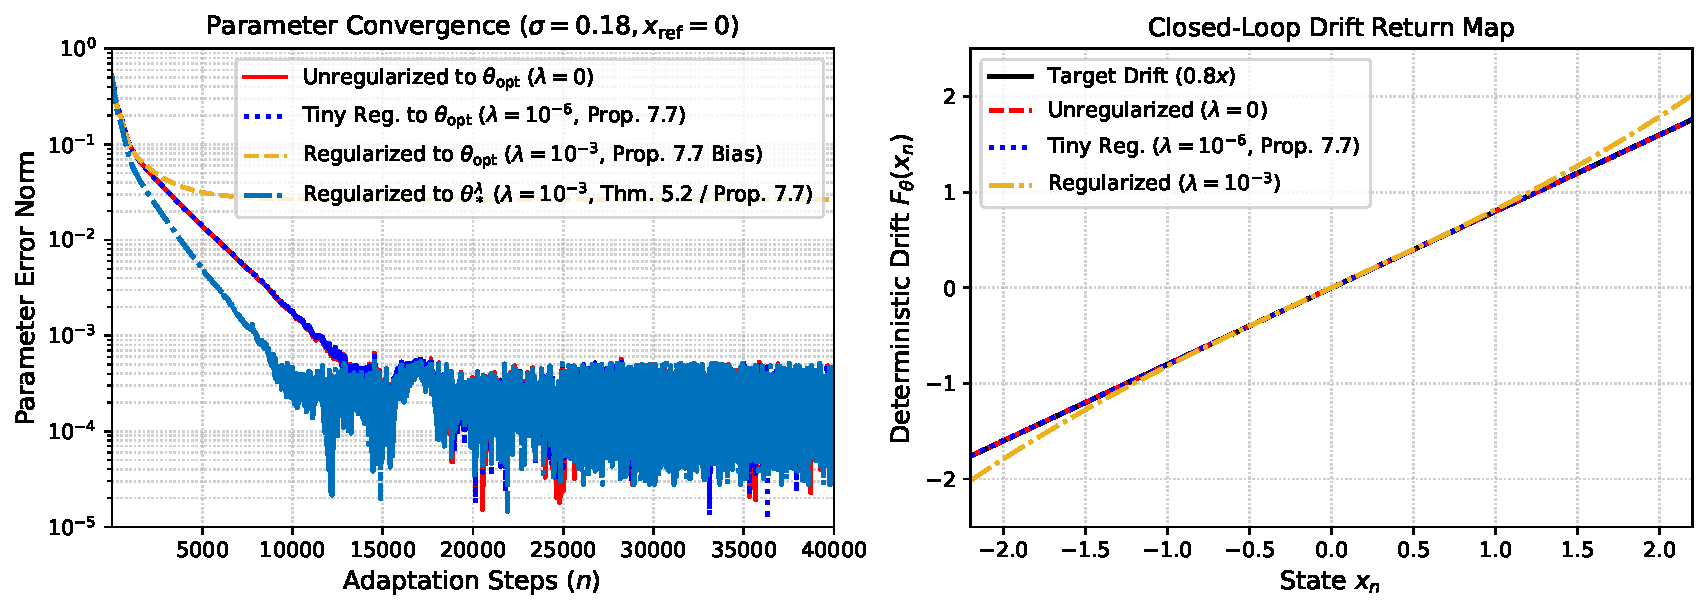
\includegraphics[width=\textwidth]{fig_part1_nominal_convergence.pdf}
\caption{Convergence of autonomous adaptation ($\sigma=0.18$, $\delta=0.10$). (Left) Parameter error. The trajectories for $\lambda=0$ (solid red) and $\lambda=10^{-6}$ (dotted blue) decay to the numerical floor. For $\lambda=10^{-3}$, the distance to $\theta_{\rm opt}$ (dashed yellow) settles at $\norm{\theta_*^\lambda - \theta_{\rm opt}} \approx 2.66\times 10^{-2}$, whereas the distance to $\theta_*^\lambda$ (dash-dotted blue) decays to the numerical floor. (Right) Return map of the deterministic drift. The unregularized (dashed red) and $\lambda=10^{-6}$ (dotted blue) fits match $x_{\rm target}(x) = 0.8x$ (solid black), while the $\lambda=10^{-3}$ fit (dash-dotted gold) retains a cubic residual.}
\label{fig:part1_nominal_convergence}
\end{figure}

For $0<\delta<\delta_0$, Theorem~\ref{thm:local-stability} together with Proposition~\ref{prop:effective-jacobian-identification} and the numerically verified positivity of $\operatorname{sym} D\overline G_\lambda(\theta^\lambda_*)$ (Section~\ref{sec:numerical-implementation}) yields local exponential convergence to $(\mu_{\theta^\lambda_*},\theta^\lambda_*)$. The global dominance condition of Theorem~\ref{thm:duffing-main-results} is not required for these experiments. While the physical component contracts at rate $1-\varepsilon_{\mathcal U}$, the $p$ slow multipliers near $1$ satisfy
\begin{equation}
    \lambda_j^{\rm slow}(\delta) = 1 - \delta \lambda_j\bigl(\Gammahat D\overline G(\theta_*)\bigr) + o(\delta), \qquad j=1,\ldots,p,
\end{equation}
as $\delta \to 0$. This yields a slow relaxation time of order $\delta^{-1}$.

For $\lambda = 10^{-3}$ ($\Gammahat=\Id$), both the shift of the stationary measure $\mu_{\theta_*^\lambda}$ and the non-vanishing linear-response term $C_*R_*B_*$ enter the reduced Jacobian $D\overline G_\lambda(\theta_*^\lambda) = H(\theta_*^\lambda) + \lambda\Id + C_*R_*B_*$. Its eigenvalues on the $M=1{,}200$ Ulam grid are $\{0.00581,\, 0.01860,\, 0.10227,\, 1.01054\}$. Because $C_* \neq 0$, the coupled linearization $\mathcal{A}_\delta$ in \eqref{eq:block-matrix} is not upper block-triangular. Thus, the small-$\delta$ expansion above and the value $\lambda_{\max}(D\overline G_\lambda(\theta_*^\lambda)) \approx 1.0105$ do not alone determine the stability threshold at finite $\delta$ (unlike the unregularized realizable setting $C_*=0$ of Section~\ref{sec:loss-of-stability}, where $\delta_c = 2/\lambda_{\max}(H_*)$ holds exactly).

To determine the finite-$\delta$ stability boundary of the discretized pair dynamics directly, we restrict $P_*$ and $B_*$ to the $(M-1)$-dimensional zero-mass subspace $V(X)$ on the $M=1{,}200$ Ulam grid (where $r(P_*\vert_{V(X)}) \approx 0.8002$). We compute the spectrum of the $(M+3)\times(M+3)$ coupled block matrix
\[
    \mathcal{A}_\delta = \begin{pmatrix} P_*\vert_{V(X)} & B_* \\ -\delta C_* & \Id - \delta\bigl(H(\theta_*^\lambda) + \lambda\Id\bigr) \end{pmatrix}.
\]
Its spectral radius satisfies $r(\mathcal{A}_\delta) \in \{0.99997,\, 0.99988,\, 0.99971,\, 0.99954\} < 1$ across the stable learning rates $\delta \in \{0.005, 0.02, 0.05, 0.08\}$. At $\delta=2.02$, $r(\mathcal{A}_{2.02}) \approx 1.0385 > 1$, crossing unity via bisection through a real eigenvalue $-1.00000006 \in \R$ at the critical threshold $\delta_c(\mathcal{A}_\delta) \approx 1.981814$. Because $\det(\mathcal{A}_\delta + \Id) = 0$ at $z=-1$ reduces via the Schur complement on $V(X)$ to $\det\bigl(2\Id - \delta M_{\rm flip}\bigr) = 0$ with
\[
    M_{\rm flip} := K - C_*\vert_{V(X)}\bigl(\Id + P_*\vert_{V(X)}\bigr)^{-1} B_*\vert_{V(X)},
    \qquad
    K := H(\theta_*^\lambda) + \lambda\Id,
\]
where $\lambda_{\max}(M_{\rm flip}) \approx 1.009176$, this threshold coincides to seven significant digits with the exact flip formula $\delta_{c,{\rm flip}} = 2/\lambda_{\max}(M_{\rm flip}) \approx 1.981814$. This lies within $0.01\%$ of $2/\lambda_{\max}(K) \approx 1.9817$ and $0.14\%$ of the adiabatic estimate $2/\lambda_{\max}(D\overline G_\lambda(\theta_*^\lambda)) \approx 1.9791$.

Figure~\ref{fig:part1_timescale_and_reg} (left) plots the empirical trajectories across $\delta \in \{0.005, 0.02, 0.05, 0.08, 2.02\}$. Figure~\ref{fig:part1_timescale_and_reg} (right) plots convergence at $\delta=0.05$. The $\lambda=10^{-3}$ trajectory converges to $\theta_*^\lambda$ faster than the unregularized trajectory ($\lambda=0$) converges to $\theta_{\rm opt}$. This reflects the increased minimum eigenvalue of the full reduced Jacobian $D\overline G_\lambda(\theta_*^\lambda)$ relative to $D\overline G(\theta_{\rm opt}) = Q_{\rm opt}$. On the Ulam grid, this eigenvalue increases from $4.06\times 10^{-3}$ to $5.81\times 10^{-3}$ (asymptotic per-step decay rates $\delta\lambda_{\min}$ increasing from $2.03\times 10^{-4}$ to $2.90\times 10^{-4}$). In the finite-horizon empirical estimate, it increases from $4.86\times 10^{-3}$ to $7.82\times 10^{-3}$. This acceleration is driven jointly by the broadened stationary distribution $\mu_{\theta_*^\lambda}$ in $H(\theta_*^\lambda)$, the $+\lambda\Id$ regularization shift, and the linear-response contribution $C_*R_*B_*$.

\begin{figure}[htpb]
\centering
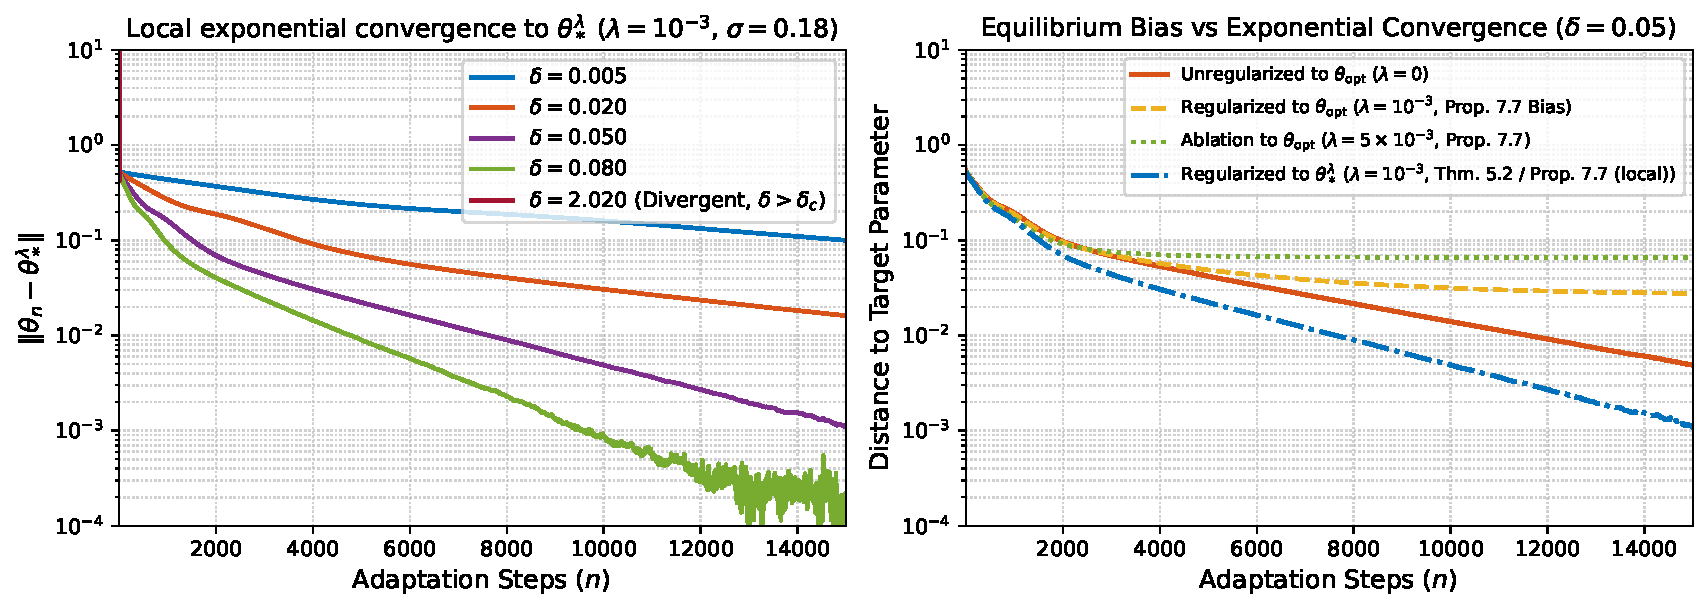
\includegraphics[width=\textwidth]{fig_part1_timescale_and_reg.pdf}
\caption{Local exponential convergence to $\theta_*^\lambda$ ($\sigma=0.18$). (Left) Regularized error $\norm{\theta_n - \theta_*^\lambda}$ for $\lambda = 10^{-3}$. For $\delta < \delta_c$, trajectories converge with decay slopes proportional to $\delta$. For $\delta=2.02 > \delta_c$, the trajectory diverges. (Right) Convergence at $\delta=0.05$. Measured relative to $\theta_{\rm opt}$, trajectories settle at $O(\lambda)$ bias plateaus ($\approx 2.66\times 10^{-2}$ for $\lambda=10^{-3}$, dashed yellow; $\approx 6.64\times 10^{-2}$ for $\lambda=5\times 10^{-3}$, dotted green). Measured relative to $\theta_*^\lambda$, the $\lambda=10^{-3}$ trajectory (dash-dotted blue) converges exponentially.}
\label{fig:part1_timescale_and_reg}
\end{figure}

\subsubsection{Isolating the Statistical Linear-Response Contribution \texorpdfstring{$C_*R_*B_*$}{C*R*B*}}
\label{sec:linear-response-experiment}

In the cubic achievable setting with $\lambda=0$, exact cancelation $g(\cdot,\theta_{\rm opt})=d$ implies $\nabla_\theta\ell_0(\cdot,\theta_{\rm opt})\equiv 0$ and therefore $C_*=0$. To isolate the statistical feedback term $C_*R_*B_*$ in Proposition~\ref{prop:effective-jacobian-identification}, we consider an under-parameterized quadratic compensator
\begin{equation}
    \psi_{\rm mis}(x) = [1,\, x,\, x^2]^{\mathsf T} \in \R^3, \qquad \lambda = 0,
\end{equation}
controlling the same reflected noisy cubic control system ($d(x)=0.15x^3$) at $\sigma=0.24$. Because $x^3 \notin \operatorname{span}(\psi_{\rm mis})$, the equilibrium misfit $g(\cdot,\theta_*)-d$ is nonzero at the self-consistent root $\theta_* \approx [0,\, 0.1121,\, 0]^{\mathsf T}$ of $\overline G(\theta_*)=0$. Here, parity symmetry of $\mu_{\theta_*}$ decouples the even and odd coordinates, yielding $\theta_{*,1} = 0.15\,m_4(\theta_*)/m_2(\theta_*)$.

Along the odd parameter coordinate $\theta_1$ (the linear feedback gain in $\theta=[\theta_0,\theta_1,\theta_2]^{\mathsf T}$, corresponding to the $(2,2)$ matrix entry), the frozen-measure Hessian and the full reduced Jacobian satisfy
\begin{equation}
    (H_*)_{22} = m_2(\theta_*),
    \qquad
    \bigl(D\overline G(\theta_*)\bigr)_{22}
    = (H_*)_{22} + (C_*R_*B_*)_{22}
    = m_2(\theta_*) + \theta_{*,1}m_2'(\theta_*) - 0.15\,m_4'(\theta_*),
\end{equation}
where primes denote derivatives with respect to $\theta_1$ evaluated at $\theta_*$. Using $\theta_{*,1} = 0.15\,m_4(\theta_*)/m_2(\theta_*)$, the linear-response contribution can be written in terms of the relative moment sensitivities as
\begin{equation}
    (C_*R_*B_*)_{22}
    = 0.15\,m_4(\theta_*)
      \left(
        \frac{m_2'(\theta_*)}{m_2(\theta_*)}
        - \frac{m_4'(\theta_*)}{m_4(\theta_*)}
      \right).
    \label{eq:CRB22-relative-moments}
\end{equation}

Increasing $\theta_1$ strengthens the linear restoring drift $0.8-\theta_1$, contracting $\mu_\theta$ toward the origin so that both $m_2'(\theta_*) < 0$ and $m_4'(\theta_*) < 0$. By \eqref{eq:CRB22-relative-moments}, $(C_*R_*B_*)_{22} > 0$ holds if and only if the fourth moment contracts more rapidly than the second moment in relative terms ($\lvert m_4'(\theta_*)\rvert/m_4(\theta_*) > \lvert m_2'(\theta_*)\rvert/m_2(\theta_*)$). Under a Gaussian closure approximation where $m_4 = 3 m_2^2$, logarithmic differentiation yields $m_4'/m_4 = 2 m_2'/m_2$. This immediately implies $(C_*R_*B_*)_{22} = -0.15\,m_4\,(m_2'/m_2) > 0$. The true invariant measure deviates from Gaussianity due to the cubic drift and boundary reflections. It exhibits an equilibrium kurtosis of $m_4/m_2^2 \approx 4.98$ (compared to $3.0$ for a Gaussian), but preserves the positive sign of the feedback term. Furthermore, the misspecified deterministic drift $F_{\theta_*}(x) = (0.8 - \theta_{*,1})x + 0.15 x^3$ possesses unstable fixed points for the forward map ($F_{\theta_*}'(x_u) \approx 1.62 > 1$) at $x_u = \pm\sqrt{(0.20 + \theta_{*,1})/0.15} \approx \pm 1.44$. Beyond these points, deterministic trajectories are repelled toward the reflecting boundaries at $\pm 2$.

To evaluate these operators and verify this relative contraction condition numerically, we partition $X=[-2,2]$ into $M$ uniform cells of width $\Delta x = 4/M$ centered at midpoints $\{x_i\}_{i=1}^M$. The discretized transfer matrix $P_\theta \in \R^{M\times M}$ is assembled by evaluating the folded Gaussian transition density between cell midpoints across the reflection branches of $\mathfrak{r}_2$ and normalizing columns to unit mass. The stationary distribution $\mu_\theta \in \R^M$ is obtained by solving $(\Id - P_\theta)\mu_\theta = 0$ subject to $\mathbf{1}^{\mathsf T}\mu_\theta = 1$, and $\theta_*$ is computed by Newton iteration on $\overline G(\theta)=0$. At $\theta_*$, the sensitivity columns $B_* e_j = (D_\theta P_{\theta_*}[e_j])\mu_*$ ($j=1,2,3$) are evaluated by differentiating the folded Gaussian kernel analytically with respect to the drift along $\partial_{\theta_j} F_\theta = -\psi_{\rm mis,j}$ and subtracting $(\mathbf{1}^{\mathsf T} B_* e_j)\mu_*$ so that $B_* e_j$ lies in the zero-mass subspace $V(X) = \{\eta \in \R^M : \mathbf{1}^{\mathsf T}\eta = 0\}$. The resolvent action $R_* B_* = (\Id - P_*)^{-1}\vert_{V(X)} B_*$ is obtained by solving the nonsingular rank-one stabilized linear system
\[
    \bigl(\Id - P_* + \mu_* \mathbf{1}^{\mathsf T}\bigr)(R_* B_*) = B_*
\]
and re-projecting each column onto $V(X)$. Finally, $C_* R_* B_*$ is evaluated by integrating the equilibrium residual $(g(x_i,\theta_*) - d(x_i))\psi_{\rm mis}(x_i)$ against $R_* B_*$.

At $M=1{,}200$, the equilibrium moments and their derivatives along $\theta_1$ (computed via $D_{\theta_1}\mu_{\theta_*} = R_* B_* e_2$) are $m_2(\theta_*) \approx 0.1500$, $m_4(\theta_*) \approx 0.1121$, $m_2'(\theta_*) \approx -1.1313$, and $m_4'(\theta_*) \approx -2.2809$. This gives relative sensitivities
\[
    \frac{m_2'(\theta_*)}{m_2(\theta_*)} \approx -7.5398,
    \qquad
    \frac{m_4'(\theta_*)}{m_4(\theta_*)} \approx -20.3384,
\]
confirming numerically that $m_4$ contracts roughly $2.7$ times faster in relative terms than $m_2$ and yielding
\[
    (H_*)_{22} \approx 0.1500, \qquad (C_*R_*B_*)_{22} \approx +0.2153 \quad (+143.5\%), \qquad \bigl(D\overline G(\theta_*)\bigr)_{22} \approx 0.3653.
\]
On the even subspace $\operatorname{span}\{1,x^2\}$, the non-symmetric feedback block $(C_*R_*B_*)_{\rm even} \approx \bigl(\begin{smallmatrix} -0.0052 & 0.1086 \\ 0.5413 & 0.3585 \end{smallmatrix}\bigr)$ has real eigenvalues $\{-0.1265,\, +0.4797\}$, and the smallest eigenvalue of the even block increases from $\lambda_{\min}(H_{\rm even}) \approx 0.0875$ to $\lambda_{\min}(H_{\rm even} + (C_*R_*B_*)_{\rm even}) \approx 0.2352$ ($+168.9\%$). Comparing grids with $M \in \{600,\, 1{,}200,\, 2{,}400\}$ cells confirms that all reported equilibrium coordinates, moments, and eigenvalues vary by less than $10^{-5}$ across resolutions. 

As an independent consistency check on the $M=1{,}200$ grid, approximating $D\overline G(\theta_*)$ by central finite differences $[\overline G(\theta_*+\varepsilon e_j)-\overline G(\theta_*-\varepsilon e_j)]/(2\varepsilon)$ with step $\varepsilon=10^{-6}$ (re-solving $(\Id - P_{\theta_*\pm\varepsilon e_j})\mu_{\theta_*\pm\varepsilon e_j}=0$ at each perturbed parameter) matches the analytical linear-response sum $H_* + C_*R_*B_*$ to $\norm{D_{\rm FD}\overline G(\theta_*) - (H_*+C_*R_*B_*)}_2 \approx 1.19\times 10^{-8}$ (relative error $9.1\times 10^{-9}$). Omitting $C_*R_*B_*$ leaves the discrepancy $\norm{D_{\rm FD}\overline G(\theta_*) - H_*}_2 \approx 0.6517$ (for the regularized cubic system of Section~\ref{sec:part1-illustration} at $\lambda=10^{-3}$ and $\sigma=0.18$, the corresponding finite-difference error is $\norm{D_{\rm FD}\overline G_\lambda(\theta_*^\lambda) - (H(\theta_*^\lambda)+\lambda\Id+C_*R_*B_*)}_2 \approx 2.04\times 10^{-9}$ versus $\norm{D_{\rm FD}\overline G_\lambda(\theta_*^\lambda)-(H(\theta_*^\lambda)+\lambda\Id)}_2 \approx 7.28\times 10^{-3}$). Figure~\ref{fig:linear_response_contribution} shows that the local exponential decay of $\norm{\theta_n - \theta_*}$ under $\Phi_\delta$ ($\delta=0.05$, with the finite-$N$ ensemble driven directly by the exact empirical residual $\frac{1}{N}\sum_{i=1}^N (g(x_n^{(i)},\theta_n)-d(x_n^{(i)}))\psi_{\rm mis}(x_n^{(i)})$ so as to eliminate boundary-reflection bias at $\sigma=0.24$) follows the full linear-response rate $\lambda_j(H_* + C_*R_*B_*)$, with log-linear fitted slopes matching $\log(1-\delta\lambda_j(H_*+C_*R_*B_*))$ ($\approx -0.0184$ odd, $-0.0118$ even). The frozen-distribution approximation $\lambda_j(H_*)$ ($\approx -0.0075$ odd, $-0.0044$ even) systematically underestimates the relaxation rate.

\begin{figure}[htpb]
\centering
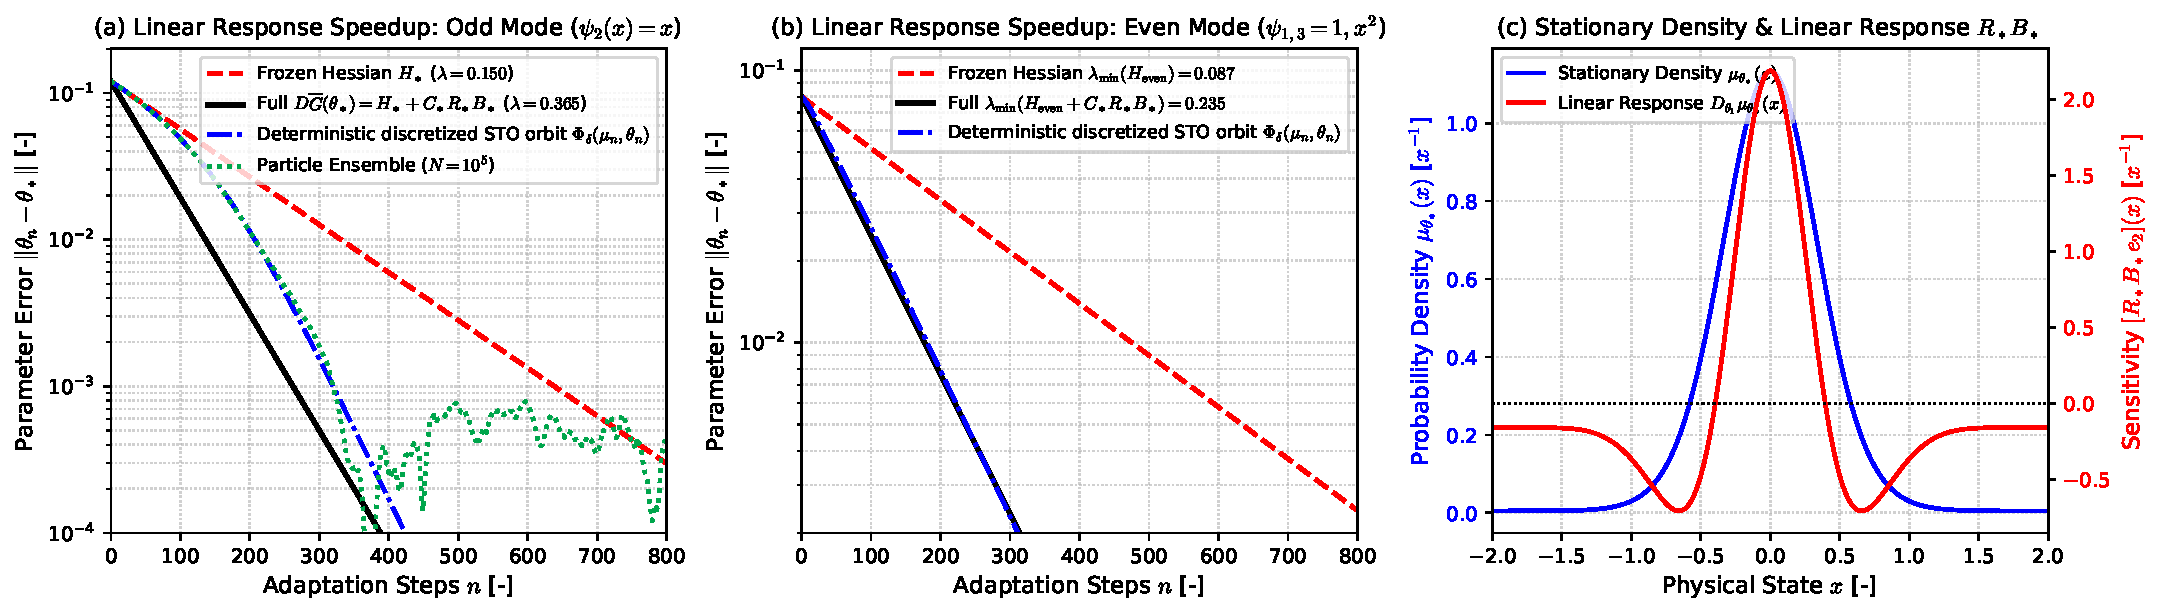
\includegraphics[width=\textwidth]{fig_linear_response_contribution.pdf}
\caption{Effect of the statistical linear-response term $C_*R_*B_*$ for the misspecified quadratic compensator $\psi_{\rm mis}(x)=[1,x,x^2]^{\mathsf T}$ ($\sigma=0.24$, $\delta=0.05$, $\lambda=0$; all quantities dimensionless). \textbf{(a)} Relaxation of the dimensionless parameter error $\norm{\theta_n - \theta_*}$ versus adaptation step $n$ for an odd-mode perturbation ($\theta_1$). The empirical finite-particle trajectory ($N=10^5$, dotted green, evaluated with the exact residual $g-d$ to exclude reflection bias) and deterministic discretized STO orbit (dash-dotted blue) match the full Jacobian decay parameter $(H_*+C_*R_*B_*)_{22} \approx 0.365$ (solid black; $0.3653$ unrounded), whereas the frozen-measure parameter $(H_*)_{22} \approx 0.150$ (dashed red; $0.1500$ unrounded) systematically underpredicts convergence. \textbf{(b)} Relaxation of $\norm{\theta_n - \theta_*}$ versus step $n$ along the slowest even mode in $\mathrm{span}\{1,x^2\}$, comparing the deterministic discretized STO orbit (dash-dotted blue) against the full Jacobian parameter $\lambda_{\min}(H_{\rm even}+(C_*R_*B_*)_{\rm even}) \approx 0.235$ (solid black; $0.2352$ unrounded) and the frozen-measure parameter $\lambda_{\min}(H_{\rm even}) \approx 0.087$ (dashed red; $0.0875$ unrounded). \textbf{(c)} Stationary density of $\mu_{\theta_*}$ (left axis, blue) and its linear response $D_{\theta_1}\mu_{\theta_*}=R_*B_*e_2$ (right axis, red), where $e_2=(0,1,0)^{\mathsf T}$. The perturbation $\theta_1\mapsto\theta_1+\varepsilon$ changes the physical drift by $-\varepsilon x$, with the other coefficients and the noise law held fixed. Relative to the dotted zero-response line, the response is positive near the origin and negative farther away, indicating increased concentration for positive $\varepsilon$.}
\label{fig:linear_response_contribution}
\end{figure}

\subsection{Part 2: Ill-Conditioning, Deployment Mismatch, and Large Learning Rates}
\label{sec:part2-practice}

Real-world adaptive and learning-based control systems often operate outside ideal hypotheses. In robotic posture and exoskeleton control \cite{lippi2018prediction,lippi2021icinco}, for example, a compensator is commonly pre-trained offline on data collected with a high-gain stabilizing baseline controller. It is subsequently released into online adaptation under a more compliant gain, operating over finite time horizons and with finite learning rates \cite{LippiActionError}. The experiments in this subsection place our mathematical framework within this broader applied context, showing how the operator-theoretic quantities explain three characteristic phenomena:
\begin{enumerate}[label=(\roman*)]
    \item \emph{Finite-horizon ill-conditioning vs.\ asymptotic stability (Section~\ref{sec:weak-excitation}):} For any $\sigma>0$, Proposition~\ref{prop:duffing-doeblin} and Remark~\ref{rem:duffing-realizable-case} guarantee $H_*\succ 0$ and asymptotic exponential convergence. In practice, however, small noise ($\sigma=0.10$) causes $\lambda_{\min}(H_*)\propto \sigma^6$ to nearly vanish. This illustrates the classical tension between regulation and persistent excitation \cite{AnnaswamyFradkov2021,Annaswamy2023,LippiActionError} as a severe finite-time bottleneck outside the core of $\mu_*$.
    \item \emph{Non-local transient recovery from deployment mismatch (Section~\ref{sec:deployment-invariance-failure}):} Theorem~\ref{thm:local-stability} establishes stability in a local neighborhood $\mathcal N_\delta$ of $(\mu_*,\theta_*)$. In contrast, deploying an offline-trained controller $\theta_{\rm off}$ with a nonzero invariance residual $\mathfrak R_A = P_{\theta_{\rm off}}\mu_{\rm off}-\mu_{\rm off}\neq 0$ drives an immediate distributional shift into out-of-distribution states \cite{LippiActionError,sinha2023systemlevelviewoutofdistributiondata,kang2022lyapunovdensitymodelsconstraining}. This initializes the pair dynamics far from equilibrium and triggers a macroscopic transient shift ($\mu_{\rm off}\to\mu_{\rm deploy}$) before online adaptation restores convergence to $(\mu_*,\theta_*)$.
    \item \emph{Large learning rates and post-instability dynamics (Section~\ref{sec:loss-of-stability}):} Whereas Theorem~\ref{thm:local-stability} holds for $0<\delta<\delta_0$, testing the upper limits of the learning rate across and beyond the linear stability threshold $\delta_c = 2/\lambda_{\max}(H_*)$ reveals damped alternating density oscillations, a nonlinear period-$2$ saturation regime, and a secondary breakdown of physical contractivity.
\end{enumerate}

\subsubsection{Weak Excitation and Ill-Conditioning}
\label{sec:weak-excitation}
Gaussian noise of intensity $\sigma > 0$ ensures $\mu_*$ has full support on $X=[-2,2]$ and the polynomial features remain linearly independent ($H_* \succ 0$). However, reducing $\sigma$ to $0.10$ lowers $\lambda_{\min}(H_*)$ to $\approx 1.29\times 10^{-4}$ via \eqref{eq:duffing-sigma6-law}. Because $\mu_*$ concentrates tightly near the origin (Figure~\ref{fig:part2_identifiability_trap_pe}, left), higher-order monomials become nearly collinear with respect to $L^2(\mu_*)$, rendering $H_*$ severely ill-conditioned. The slowest multiplier approaches $1$ (with relaxation time $1/(\delta\lambda_{\min}(H_*)) \approx 7.8\times 10^4$ steps at $\delta=0.10$), slowing parameter convergence over finite horizons. Consequently, at $n=40{,}000$ steps (Figure~\ref{fig:part2_identifiability_trap_pe}, right), the compensator matches the target drift near the origin but retains large errors in regions of low stationary probability.

\begin{figure}[htpb]
\centering
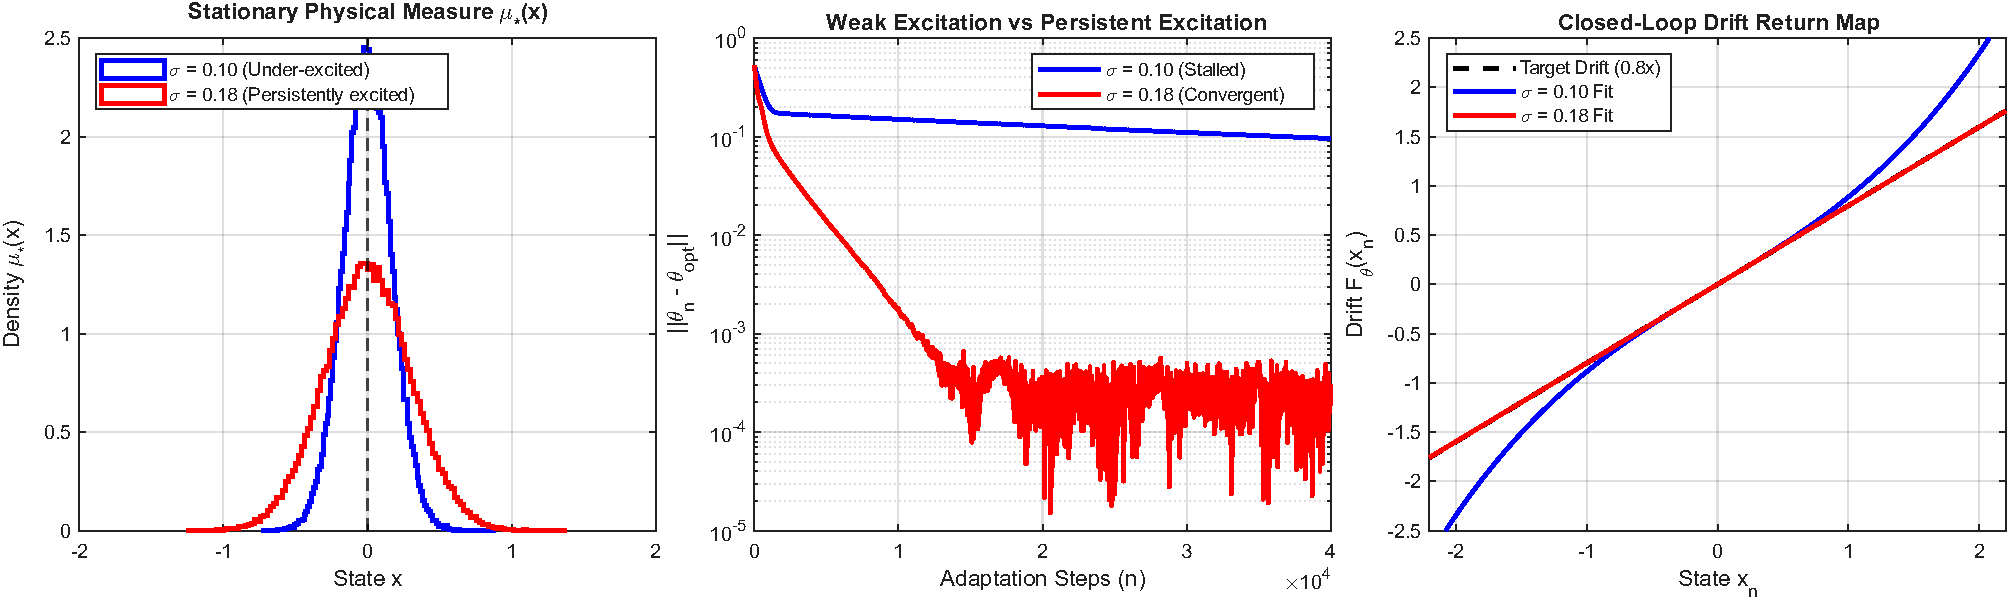
\includegraphics[width=\textwidth]{fig_part2_identifiability_trap_pe.pdf}
\caption{Weak excitation and ill-conditioning ($\delta=0.10$). (Left) Stationary distribution $\mu_*(x)$. At $\sigma=0.10$, the density concentrates near $x=0$. (Middle) Parameter error $\norm{\theta_n - \theta_{\rm opt}}$. At $\sigma=0.10$, $\lambda_{\min}(H_*) \approx 1.29\times 10^{-4}$, stalling convergence. (Right) Return map of the deterministic drift. For $\sigma=0.10$, the fit matches $0.8x$ near the origin but diverges outside $[-0.5, 0.5]$.}
\label{fig:part2_identifiability_trap_pe}
\end{figure}

\subsubsection{Failure of Invariance at Deployment}
\label{sec:deployment-invariance-failure}
In the two-phase deployment protocol ($\lambda=0$), we perform offline pre-training under the conservative baseline controller $u_{\rm base}^{\rm off}(x) = -0.80x$ at noise intensity $\sigma_{\rm off}=0.10$. The parameter update evaluates the unchanged tracking-error residual $-(x_{n+1}-0.8x_n)$ of \eqref{eq:empirical-tracking-gradient} relative to the nominal reference model $0.8x_n$. Because the pre-reflection dynamics under $u_{\rm base}^{\rm off}(x)=-0.80x$ is
\[
    x_{n+1} = 0.25x_n + d(x_n) - g(x_n,\theta) + \xi_n,
\]
neglecting boundary reflection and using centered noise ($\mathbb{E}[\xi_n]=0$) yields the conditional expectation $\mathbb{E}[-(x_{n+1}-0.8x_n)\mid x_n=x] = g(x,\theta) - d(x) + 0.55x$. Up to the negligible reflection tail, the offline update therefore follows the gradient of the shifted quadratic loss
\[
    \ell_{\rm off}(x,\theta) = \frac{1}{2}\bigl(g(x,\theta) - d(x) + 0.55x\bigr)^2,
\]
corresponding to the offline learning field
\begin{equation}
    G_{\rm off}(\mu,\theta) := \int_X \bigl(g(x,\theta) - d(x) + 0.55x\bigr)\psi(x)\,\dd\mu(x).
    \label{eq:offline-learning-field}
\end{equation}
Offline identification under the offline transfer operator $P_{\rm off,\theta}$ thus seeks $\theta_{\rm off}$ such that
\begin{equation}
    G_{\rm off}(\mu_{\rm off}, \theta_{\rm off}) \approx 0.
\end{equation}
By Proposition~\ref{prop:all-fixed-points}, equilibrium after deployment under the relaxed baseline gain $u_{\rm base}^{\rm dep}(x) = -0.25x$ requires instead
\begin{equation}
    P_{\rm dep,\theta_*}\mu_* = \mu_* \qquad \text{and} \qquad G_{\rm dep}(\mu_*,\theta_*) = 0,
\end{equation}
where $P_{\rm dep,\theta} \equiv P_\theta$ and $G_{\rm dep}(\mu,\theta) \equiv G(\mu,\theta) = \int_X (g(x,\theta)-d(x))\psi(x)\,\dd\mu(x)$. Relaxing the baseline gain from $-0.80x$ to $-0.25x$ therefore modifies both the physical transition kernel ($P_{\rm off,\theta}\mapsto P_{\rm dep,\theta}$) and the effective target of the learning rule ($d(x)-0.55x \mapsto d(x)$). In the unregularized realizable cubic polynomial case, exact offline identification ($G_{\rm off}(\mu_{\rm off},\theta_{\rm off}^*)=0$, neglecting reflection) would yield the ideal offline compensator
\[
    g_{\rm off}^*(x) = 0.15x^3 - 0.55x, \qquad \theta_{\rm off}^* = [0,\, -0.55,\, 0,\, 0.15]^{\mathsf T}.
\]
Upon deployment under $u_{\rm base}^{\rm dep}(x)=-0.25x$, the deterministic map before reflection becomes
\begin{equation}
    F_{\rm dep}(x) := 0.8x + 0.15x^3 - g(x,\theta),
    \label{eq:F-dep-general}
\end{equation}
which for the ideal offline compensator $g_{\rm off}^*$ reduces to $F_{\rm dep}(x) = 0.8x + 0.15x^3 - g_{\rm off}^*(x) = 1.35x$. Thus, even exact offline identification with respect to the fixed reference residual $x_{n+1}-0.8x_n$ produces a compensator that destabilizes the origin once the baseline gain is relaxed.

If the deployed transfer operator $P_{\rm dep,\theta_{\rm off}} \equiv P_{\theta_{\rm off}}$ does not preserve $\mu_{\rm off}$, physical invariance fails, yielding the residual \cite{LippiActionError}:
\begin{equation}
    \mathfrak{R}_A := P_{\rm dep,\theta_{\rm off}}\mu_{\rm off} - \mu_{\rm off} \neq 0.
    \label{eq:action-residual-ref}
\end{equation}
We distinguish two quantities. The invariance residual $\mathfrak{R}_A = P_{\rm dep,\theta_{\rm off}}\mu_{\rm off}-\mu_{\rm off}\in V(X)$ is a signed measure. It vanishes if and only if $\mu_{\rm off}$ is invariant for the deployed kernel, and it drives the transient shift $\mu_{\rm off}\to\mu_{\rm deploy}$. The compensation error $\mathcal{E}_A(\theta_n)=\norm{g(\cdot,\theta_n)-d}_{L^2(\mu_n)}$ in \eqref{eq:empirical-compensation-error} measures the mismatch of the compensator on the current state distribution. Figure~\ref{fig:part2_action_error_recovery} (middle) reports $\mathcal{E}_A(\theta_n)$, not $\mathfrak{R}_A$.

In the finite-horizon simulation ($3{,}000$ pre-training steps from $\theta_{\rm off,0}=[0,-0.45,0,0.28]^{\mathsf T}$ and $x_0^{(i)}=0$ at $\delta_{\rm off}=0.002$, $\sigma_{\rm off}=0.10$, and regularization $\lambda=0$), pre-training under $u_{\rm base}^{\rm off}(x) = -0.80x$ confines $\mu_{\rm off}$ near the origin ($\operatorname{std}_{\mu_{\rm off}}(X)\approx 0.141$, $\lambda_{\min}(H(\mu_{\rm off}))\approx 4.49\times 10^{-5}$; Figure~\ref{fig:part2_action_error_recovery}, left). Consequently, the linear coefficient adapts partially toward $-0.55$ while the higher-order cubic coefficient is poorly excited and remains near its initialization. This yields the learned parameter vector
\begin{equation}
    \theta_{\rm off} = [\theta_{0,\rm off},\, \theta_{1,\rm off},\, \theta_{2,\rm off},\, \theta_{3,\rm off}]^{\mathsf T} \approx [1.03\times 10^{-5},\, -0.46188,\, 4.62\times 10^{-7},\, 0.27928]^{\mathsf T}.
    \label{eq:theta-off-numerical}
\end{equation}
Substituting \eqref{eq:theta-off-numerical} into \eqref{eq:F-dep-general} gives the deployed pre-reflection map
\[
\begin{aligned}
    F_{\rm dep}(x) &= -\theta_{0,\rm off} + (0.8 - \theta_{1,\rm off})x - \theta_{2,\rm off}x^2 + (0.15 - \theta_{3,\rm off})x^3 \\
    &\approx -1.03\times 10^{-5} + 1.26188\,x - 4.62\times 10^{-7}\,x^2 - 0.12928\,x^3,
\end{aligned}
\]
whose derivative at the origin is
\begin{equation}
    F_{\rm dep}'(0) = 0.8 - \theta_{1,\rm off} \approx 1.26188 > 1
    \label{eq:F-dep-slope}
\end{equation}
(compared to $1.35$ for the ideal offline compensator $\theta_{\rm off}^*$). Because the finite-ensemble constant term $\theta_{0,\rm off}\approx 1.03\times 10^{-5}$ is negligible, the central fixed point of $F_{\rm dep}(x)=x$ lies at $x_{\rm fp,0} \approx +3.92\times 10^{-5} \approx 0$ with multiplier $F_{\rm dep}'(x_{\rm fp,0}) \approx 1.26188 > 1$ (Figure~\ref{fig:part2_action_error_recovery}, right). At the same time, the unadapted cubic over-compensation $(0.15-\theta_{3,\rm off}) \approx -0.12928 < 0$ creates two locally stable outer fixed points at $x_{{\rm fp},\pm} \approx \pm 1.4233$ ($F_{\rm dep}'(x_{{\rm fp},\pm}) \approx 0.4762 \in (-1,1)$). These split $\mu_{\rm off}$ into the bimodal distribution $\mu_{\rm deploy}$ peaked near $\pm 1.42$ (Figure~\ref{fig:part2_action_error_recovery}, left), corresponding to $\mathfrak{R}_A \neq 0$.

To quantify $\mathfrak{R}_A$ numerically without taking the total variation directly between an atomic empirical measure and a continuous density, we evaluate the discretized invariance residual on the same $M$-cell Ulam grid ($h = 4/M$) used for the transfer operator:
\begin{equation}
    r_{A,h} := P_{{\rm dep},h}(\theta_{\rm off})\mu_{{\rm off},h} - \mu_{{\rm off},h},
    \qquad
    \norm{r_{A,h}}_{\ell^1} = \sum_{i=1}^M \bigl|(r_{A,h})_i\bigr|,
    \label{eq:discretized-rA}
\end{equation}
where $\mu_{{\rm off},h} \in \R^M$ is constructed as the unique stationary probability vector solving $(\Id - P_{{\rm off},h}(\theta_{\rm off}))\mu_{{\rm off},h}=0$, $\mathbf{1}^{\mathsf T}\mu_{{\rm off},h}=1$ under the offline kernel ($u_{\rm base}=-0.80x$, $\sigma_{\rm off}=0.10$). This is cross-checked against the cell-binned histogram $\mu_{{\rm off},h}^{\rm emp}$ of the $N=10^5$ offline ensemble ($\norm{\mu_{{\rm off},h}-\mu_{{\rm off},h}^{\rm emp}}_{\ell^1} \approx 0.0355$ at $M=1{,}200$). Holding $\theta_{\rm off}$ fixed at \eqref{eq:theta-off-numerical}, Table~\ref{tab:deployment_ablation} isolates the effect of relaxing the baseline gain ($-0.80x \to -0.25x$) from the effect of increasing the noise intensity ($\sigma: 0.10 \to 0.18$). Across grid resolutions $M \in \{600,\, 1{,}200,\, 2{,}400\}$, all Ulam values of $\norm{r_{A,h}}_{\ell^1}$ and of the asymptotic shift $\norm{\mu_{{\rm dep},h}-\mu_{{\rm off},h}}_{\ell^1}$ vary by less than $6\times 10^{-5}$ (e.g., $\norm{r_{A,h}}_{\ell^1} \in \{0.35216,\, 0.35212,\, 0.35213\}$ for the gain-only change and $\{0.54875,\, 0.54880,\, 0.54879\}$ for the simultaneous change). The ablation shows that the baseline gain relaxation alone destabilizes the origin ($F_{\rm dep}'(0)\approx 1.2619>1$), triggers the bimodal split ($\norm{\mu_{{\rm dep},h}-\mu_{{\rm off},h}}_{\ell^1}\approx 2.0000$, $\operatorname{std}_{\mu_{\rm dep}}(X)\approx 1.4139$), and increases the compensation error $\mathcal{E}_A(\theta_{\rm off})$ from $0.0640$ to $0.2842$. Increasing $\sigma$ alone under the fixed $-0.80x$ gain preserves a unimodal distribution ($F_{\rm off}'(0) = 0.25-\theta_{1,\rm off} \approx 0.7119 < 1$, $\operatorname{std}_{\mu_{\rm dep}}(X)\approx 0.2483$, $\mathcal{E}_A(\theta_{\rm off})\approx 0.1090$) and serves primarily to supply persistent excitation during online recovery.

\begin{table}[htpb]
\centering
\footnotesize
\setlength{\tabcolsep}{2.5pt}
\begin{tabular}{lccccccc}
\toprule
\textbf{Transition ($\theta_{\rm off}$ fixed)} & $u_{\rm base}$ & $\sigma$ & $\norm{r_{A,h}}_{\ell^1}$ \textbf{(Ulam/Emp.)} & $\norm{\mu_{{\rm dep},h}-\mu_{{\rm off},h}}_{\ell^1}$ & $\operatorname{std}(X)$ & $\mathcal{E}_A(\theta_{\rm off})$ & $\lambda_{\min}(H)$ \\
\midrule
Offline ref.\ ($\mu_{{\rm off},h}$) & $-0.80x$ & $0.10$ & $0$ & $0$ & $0.1409$ & $0.0640$ & $4.49\times 10^{-5}$ \\
Gain change only & $-0.25x$ & $0.10$ & $0.3521$ / $0.3528$ & $2.0000$ (bimodal) & $1.4139$ & $0.2842$ & $2.08\times 10^{-2}$ \\
Noise change only & $-0.80x$ & $0.18$ & $0.3603$ / $0.3624$ & $0.5398$ (unimodal) & $0.2483$ & $0.1090$ & $1.24\times 10^{-3}$ \\
Simultaneous change & $-0.25x$ & $0.18$ & $0.5488$ / $0.5501$ & $1.9972$ (bimodal) & $1.3898$ & $0.2825$ & $6.97\times 10^{-2}$ \\
\bottomrule
\end{tabular}
\caption{Separation of baseline gain relaxation and noise intensity change at deployment on the $M=1{,}200$ Ulam grid with $\theta_{\rm off}$ held fixed at \eqref{eq:theta-off-numerical}. The column $\norm{r_{A,h}}_{\ell^1}$ reports the one-step invariance residual \eqref{eq:discretized-rA} evaluated on the stationary Ulam vector $\mu_{{\rm off},h}$ and on the cell-binned $N=10^5$ empirical histogram $\mu_{{\rm off},h}^{\rm emp}$.}
\label{tab:deployment_ablation}
\end{table}

Under $\Phi_\delta$ ($\delta=0.04$, $\sigma=0.18$), the trajectory relaxes to $(\mu_*, \theta_*)$. The spread of $\mu_{\rm deploy}$ increases $\lambda_{\min}(H)$, restoring a contractive drift slope and driving the state to the unimodal measure $\mu_*$. As the misfit decreases, the linear-response contribution $C_*R_*B_*$ in the effective Jacobian diminishes, and $\norm{\theta_n - \theta_{\rm opt}}$ relaxes along the slow manifold on the time scale $O(1/(\delta\lambda_{\min}(H_*)))$.

\begin{figure}[htpb]
\centering
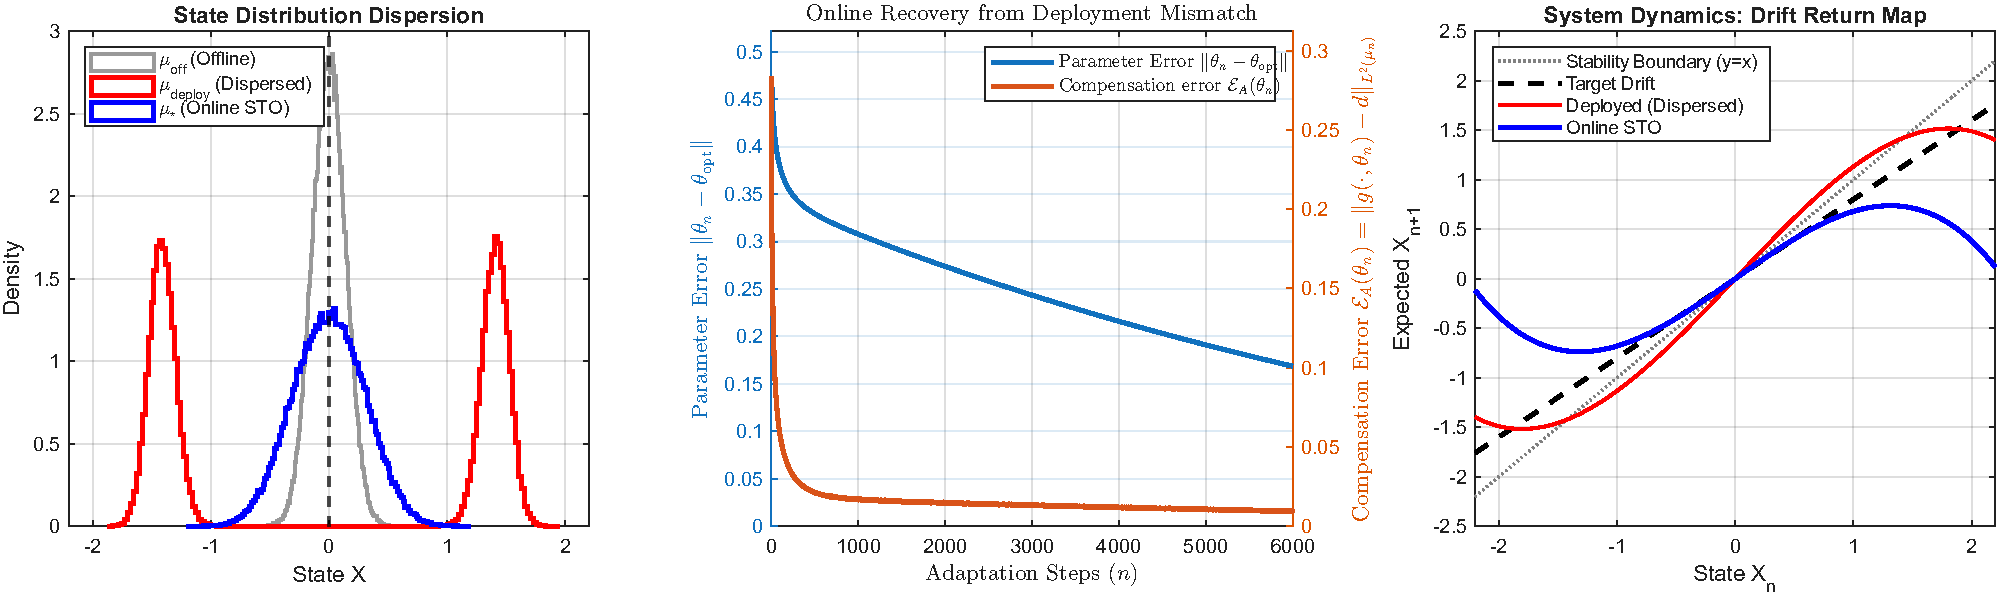
\includegraphics[width=\textwidth]{fig_part2_action_error_recovery.pdf}
\caption{Failure of invariance at deployment and online recovery ($\sigma_{\rm off}=0.10 \to \sigma_{\rm online}=0.18$, $\delta=0.04$). (Left) State distribution. High-gain pre-training ($-0.80$) produces $\mu_{\rm off}$ (gray). Relaxing the gain to $-0.25$ and increasing the noise intensity $\sigma = 0.10 \to 0.18$ (Table~\ref{tab:parameters}) act as concurrent drivers yielding $\mathfrak R_A \neq 0$ and driving the state into $\mu_{\rm deploy}$ (red). Adaptation under $\Phi_\delta$ restores contractivity and returns the state to $\mu_*$ (blue). (Middle) Error trajectories. Online adaptation reduces the compensation error $\mathcal{E}_A(\theta_n)$ (orange), after which both $\mathcal{E}_A$ and $\norm{\theta_n - \theta_{\rm opt}}$ (blue) decay along the slow manifold. (Right) Return map of the deterministic drift. The deployed drift $F_{\rm dep}$ (red) has slope $F_{\rm dep}'(0)>1$ at the origin; adaptation (blue) restores a contractive slope matching $x_{target}$ (dashed black).}
\label{fig:part2_action_error_recovery}
\end{figure}

Conversely, assume offline identification uses the deployment baseline gain ($-0.25$) and the same noise law $\mathcal{N}(0,\sigma^2)$, so that $G_{\rm off} \equiv G_{\rm dep}$. Let $\mu_{\rm off}$ denote the stationary distribution reached during a burn-in phase with the resulting controller $\theta_{\rm off}^{\rm match} \approx [-1.14\times 10^{-5},\, 0.01079,\, 3.54\times 10^{-5},\, 0.00270]^{\mathsf T}$ held frozen (for which $F_{\rm dep}'(0) = 0.8 - \theta_{1,\rm off}^{\rm match} \approx 0.7892 < 1$). Then the offline and deployed transition kernels coincide:
\begin{equation}
    P_{\rm dep,\theta_{\rm off}^{\rm match}}\mu_{\rm off} = \mu_{\rm off}, \qquad \mathfrak{R}_A = 0 \quad (\norm{r_{A,h}}_{\ell^1} = 0).
\end{equation}
Figure~\ref{fig:part2_escaping_trap_offline} confirms that under this matched protocol, the deployed distribution remains unimodal, avoiding the transient bimodal split.

\begin{figure}[htpb]
\centering
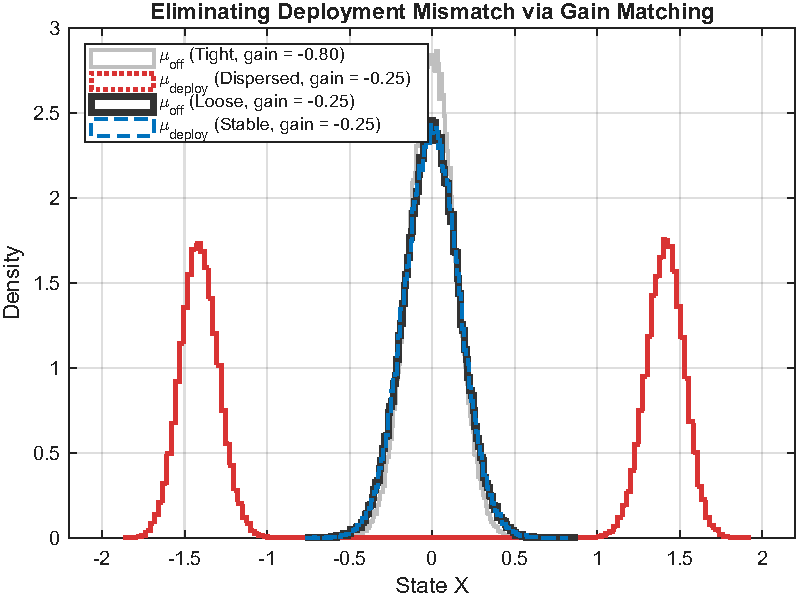
\includegraphics[width=0.7\textwidth]{fig_part2_escaping_trap_offline.pdf}
\caption{Elimination of the invariance residual \eqref{eq:action-residual-ref} at $\sigma=0.10$. Pre-training under $u_{\rm base}(x) = -0.80x$ (solid light gray) induces a kernel mismatch that splits the deployed distribution into $\mu_{\rm deploy}$ (dotted red). Pre-training under the matched baseline $u_{\rm base}(x) = -0.25x$ (solid dark charcoal) yields $\mathfrak{R}_A = 0$, so the deployed distribution (dashed blue) remains unimodal.}
\label{fig:part2_escaping_trap_offline}
\end{figure}

\subsubsection{Loss of Linear Stability and Oscillatory Behavior}
\label{sec:loss-of-stability}

In the unregularized, exactly realizable case ($\lambda=0$, $g(\cdot,\theta_{\rm opt})=d$, $\Gammahat=\Id$), the feedback block $C_*$ vanishes identically and the linearized pair operator \eqref{eq:block-matrix} is upper block-triangular:
\begin{equation}
    \mathcal{A}_\delta = \begin{pmatrix} P_* & B_* \\ 0 & \Id - \delta H_* \end{pmatrix}.
\end{equation}
Consequently, the multipliers of the parameter block are exactly $\lambda_j^{\rm slow}(\delta) = 1 - \delta \lambda_j(H_*)$ for all $\delta > 0$. The linear stability threshold is
\begin{equation}
    \delta_c = \frac{2}{\lambda_{\max}(H_*)}.
\end{equation}
The only approximation lies in the numerical estimation of $H_*$. As $\delta$ increases, the leading multiplier $1 - \delta\lambda_{\max}(H_*)$ crosses zero at $\delta_{\rm osc} := 1/\lambda_{\max}(H_*)$, producing an alternating linearized mode, and exits the unit disk through $-1$ at $\delta_c$. Crossing $-1$ indicates loss of linear stability along an alternating mode. Establishing a rigorous flip bifurcation requires additional nonlinear nondegeneracy conditions.

Figure~\ref{fig:part2_bifurcation_diagram} shows the empirical distribution of $X_n$ across $\delta \in [1.50, 2.25]$ at $\sigma=0.05$ ($\sigma_x \approx 0.0833$). At $\theta_{\rm opt}$, the eigenvalues of $H_*$ are $\lambda_1 \approx 2.01\times 10^{-6}$ ($x^3$ mode), $\lambda_2 \approx 9.64\times 10^{-5}$ ($x^2$ mode), $\lambda_3 \approx 6.95\times 10^{-3}$ ($x$ mode), and $\lambda_4 = \lambda_{\max}(H_*) \approx 1.00005$ (aligned with the constant bias feature $\psi_1(x)=1$, with eigenvector $v_4 \approx [1,0,0.0069,0]^{\mathsf T}$), yielding $\delta_c = 2/\lambda_{\max}(H_*) \approx 1.9999 \approx 2.000$ ($1.9998$ for the $N=100$ ensemble). The initial parameter perturbation $\theta_0 - \theta_{\rm opt} = [10^{-2}, -10^{-2}, 0, 0]^{\mathsf T}$ projects equally ($70.7\%$ of its Euclidean norm) onto the dominant constant-bias mode $v_4$ and the linear-gain mode $v_3$. Above $\delta_c$, one must distinguish the local loss of stability of the equilibrium from the macroscopic broadening of the state distribution visible in Figure~\ref{fig:part2_bifurcation_diagram}. On a discretization grid with step $\Delta\delta \approx 1.5\times 10^{-3}$ ($500$ points in $[1.50, 2.25]$), for $\delta \in (2.00, 2.19)$, the unstable multiplier $1 - \delta\lambda_{\max}(H_*) \in (-1.19, -1.00)$ rapidly amplifies sign-alternating perturbations along the constant offset $\theta_0$ (for instance, at $\delta=2.18$, linear growth amplifies a perturbation by $10^2$ in $\log 100/\log 1.18 \approx 28$ steps). Note that the identity $H(\mu)_{11} = \int_X 1^2\dd\mu = 1$ implies $\lambda_{\max}(H(\mu)) \ge 1$ and hence $1 - \delta\lambda_{\max}(H(\mu)) < -1$ for every $\delta > 2$; consequently, this instability cannot saturate via the Gram matrix alone. Instead, as $\theta_{0,n} \approx (-1)^n a_0$ alternates in sign, the mean physical state $m_{1,n} = \mathbb{E}_{\mu_n}[X_n] \approx \frac{a_0}{1.8 - \bar{\theta}_1}(-1)^n$ oscillates in phase with $\theta_{0,n}$. This couples the odd coefficients into the bias update $G_0(\mu_n,\theta_n) = \theta_{0,n} + \theta_{1,n}m_{1,n} + \theta_{2,n}m_{2,n} + (\theta_{3,n}-0.15)m_{3,n} \approx \bigl(1 + \frac{\bar{\theta}_1}{1.8 - \bar{\theta}_1}\bigr)\theta_{0,n}$. A negative steady shift of the linear gain ($\bar{\theta}_1 \approx -0.056$ at $\delta=2.05$, $-0.135$ at $\delta=2.15$, and $-0.166$ at $\delta=2.18$, accompanied by $\bar{\theta}_3 \approx 0.175$) reduces this effective loop gain to $2/\delta$. This saturates the primary flip instability into a bounded period-$2$ regime ($\norm{\theta_n - \theta_{\rm opt}} \approx 0.10$--$0.31$, with state excursions $\vert X_n(1)\vert \lesssim 0.08$ over $n \in [1{,}501, 1{,}600]$ that appear close to zero on the $[-2, 2]$ scale). However, because the closed-loop linear slope at the origin is $0.8 - \theta_1$, shifting $\theta_1$ negatively weakens physical contractivity: when $\delta$ exceeds the secondary threshold $\delta \approx 2.19$ ($2.1895 \pm 0.0028$ for $N=10^2$ and $2.1950 \pm 0.0000$ for $N=10^4$ across $10$ random seeds), $\theta_{1,n}$ crosses $-0.20$ (where $0.8 - \theta_{1,n} > 1$), the physical state loses contractivity, and boundary reflections drive a secondary runaway across $[-2, 2]$. Figure~\ref{fig:part2_density_shattering} compares the evolution of the state density $\mu_n(x)$ over $n \in [1, 150]$ for $\delta=1.85 \in (\delta_{\rm osc}, \delta_c)$ (where the alternating linear multiplier $\approx -0.85$ produces damped sign-alternating oscillations of the density) and $\delta=2.22 > \delta_c$ (where the unstable multiplier $\approx -1.22$ and secondary nonlinear coupling disperse the density across $[-2, 2]$).

\begin{figure}[htpb]
\centering
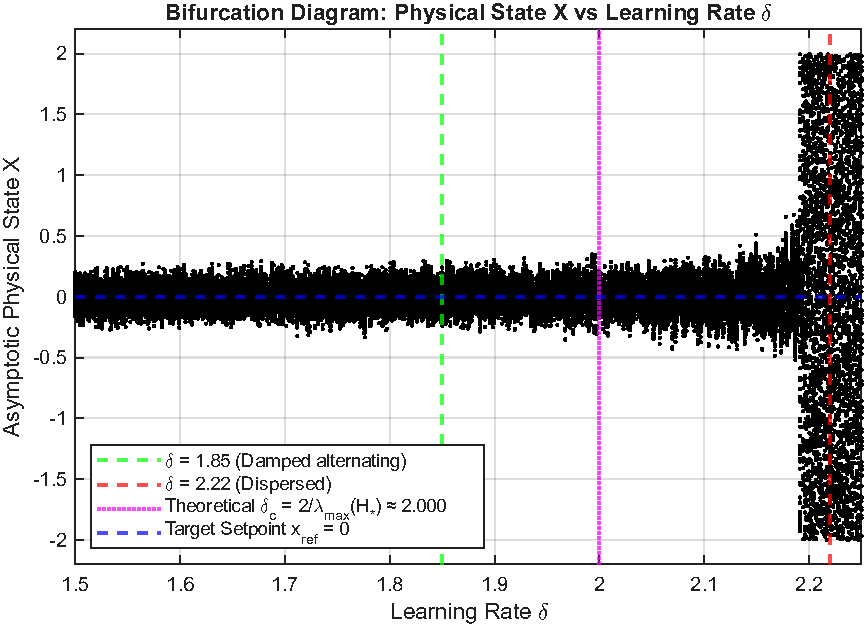
\includegraphics[width=0.7\textwidth]{fig_part2_bifurcation_diagram.pdf}
\caption{Empirical bifurcation diagram of $X_n \in [-2, 2]$ versus $\delta \in [1.50, 2.25]$ at $\sigma=0.05$. Vertical dashed lines mark $\delta=1.85$ (green) and $\delta=2.22$ (red); the dotted magenta line marks $\delta_c = 2/\lambda_{\max}(H_*) \approx 2.000$. Below $\delta_c$, the equilibrium is stable and the state remains near $x=0$ (dashed blue); for $\delta \in (\delta_c, 2.19)$, the primary instability along $\theta_0$ saturates into a bounded alternating regime (period-2 orbit) around $x=0$, whereas for $\delta \gtrsim 2.19$ (with grid step $\Delta\delta \approx 1.5\times 10^{-3}$) a secondary nonlinear instability spreads trajectories across $[-2, 2]$.}
\label{fig:part2_bifurcation_diagram}
\end{figure}

\begin{figure}[htpb]
\centering
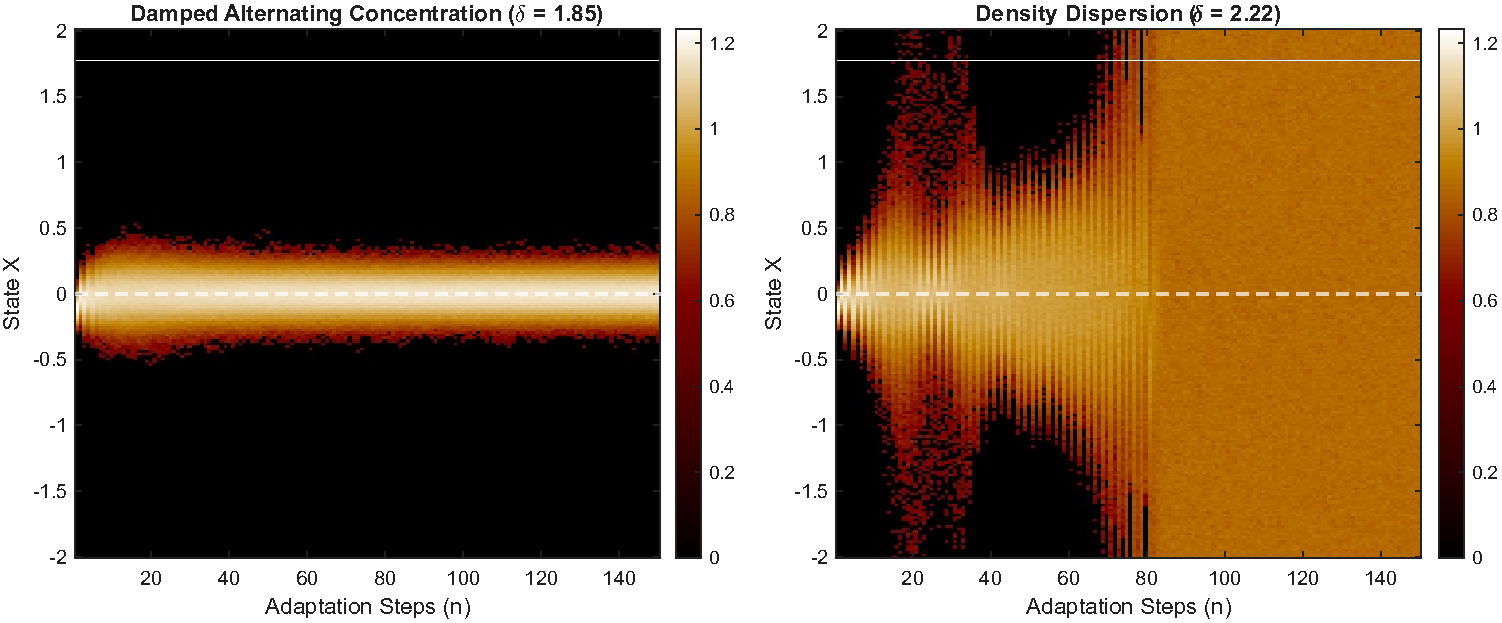
\includegraphics[width=\textwidth]{fig_part2_density_shattering.pdf}
\caption{Evolution of the state density $\mu_n(x)$ over $n \in [1, 150]$ from $\theta_0=[0.10, -0.10, 0, 0]^{\mathsf T}$ ($N=10^4, \sigma=0.05$). Color intensity shows $(\mathrm{PDF})^{0.1}$. (Left) Damped alternating regime ($\delta=1.85$). The multiplier $\approx -0.85 \in (-1,0)$ produces damped sign-alternating oscillations of the density. (Right) Supercritical regime ($\delta=2.22 > \delta_c$). The multiplier $\approx -1.22 < -1$ amplifies sign-alternating oscillations and disperses the density across $[-2, 2]$.}
\label{fig:part2_density_shattering}
\end{figure}

\subsection{Numerical Exploration of Non-Convex Neural Parameterizations}
\label{sec:nonconvex_extension}

The explicit verification of the theoretical hypotheses in Section~\ref{sec:duffing-example} concerns the fixed-feature linear-readout model $g(x,\theta)=\theta^{\mathsf T}\psi(x)$. The abstract stationary reduction and degree criterion of Section~\ref{4}, however, do not require loss landscape convexity. If the frozen dynamics admits a unique continuous stationary branch $\theta\mapsto\mu_\theta$ and the reduced field $\overline G(\theta) = G(\mu_\theta,\theta)$ satisfies $0 \notin \overline G(\partial\Omega)$ and $\deg(\overline G,\Omega,0)\neq 0$ on a bounded open set $\Omega\subset\R^p$ (Theorem~\ref{thm:degree-existence}), then $\STO_\delta$ admits an adaptive equilibrium $\rho_* = \mu_{\theta_*}\otimes\delta_{\theta_*}$. Unlike the fixed-feature linear-readout case of Proposition~\ref{prop:duffing-constructive-existence}, adapting internal network weights couples the feature sensitivities to the readout magnitude. Verifying the outward-pointing condition $\langle\overline G(\theta),\theta\rangle>0$ on large spheres requires additional estimates on the radial growth of the learning field. Unlike the linear-readout case, $\lambda\norm{\theta}^2$ alone does not control this growth because the features $\tanh(W_1x+b_1)$ themselves depend on $\theta$. We do not establish such estimates for the MLP \eqref{eq:mlp-compensator}; the experiment below is presented purely as a numerical exploration.

To explore the behavior of the coupled dynamics beyond the linear-readout setting, we replace the polynomial basis with a fully adaptive multilayer perceptron ($8$ $\tanh$ hidden units, $p=25$ parameters):
\begin{equation}
    g(x, \theta) = W_2 \tanh(W_1 x + b_1) + b_2, \qquad \theta = \mathrm{vec}(W_1, b_1, W_2, b_2) \in \R^{25}.
    \label{eq:mlp-compensator}
\end{equation}
For initial weights $\theta_0 \sim \mathcal{N}(0, 0.1^2 I_{25})$ and parameters $\delta=0.05$, $\sigma=0.10$, and $\lambda=10^{-5}$, the empirical tracking loss converges smoothly to the Gaussian noise floor $\sigma^2/2 = 0.005$ (Figure~\ref{fig:mlp_convergence}).

\begin{figure}[htpb]
\centering
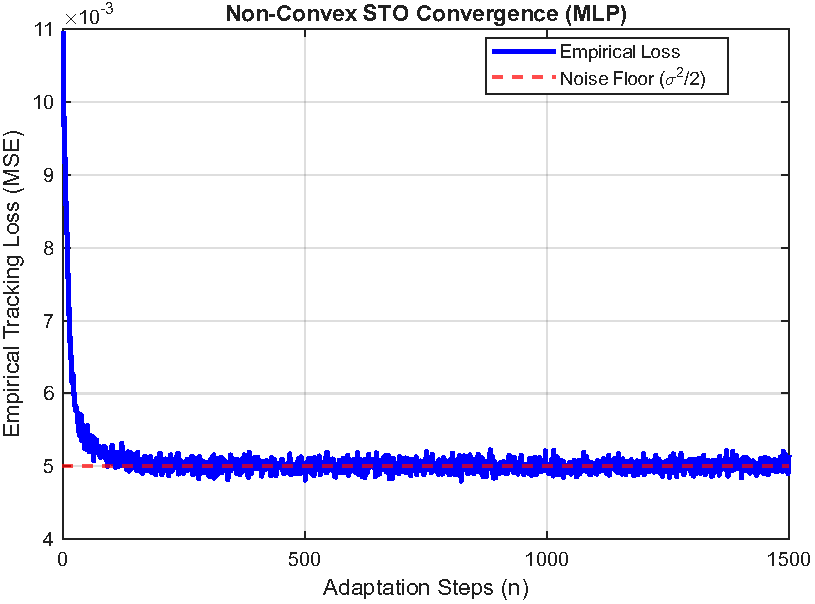
\includegraphics[width=0.7\textwidth]{fig5_mlp_convergence.pdf}
\caption{Autonomous adaptation of an MLP compensator ($p=25$, $\delta=0.05$, $\sigma=0.10$, $\lambda=10^{-5}$). The empirical tracking loss converges to the Gaussian noise floor $\sigma^2/2 = 0.005$ (dashed red).}
\label{fig:mlp_convergence}
\end{figure}

\subsection{Reproducibility Details and Algorithmic Protocols}
\label{sec:reproducibility-protocols}

Table~\ref{tab:reproducibility_vectors} summarizes the initial conditions $(x_0^{(i)},\theta_0)$, random seeds, ensemble sizes $N$, independent realizations $R$, and resulting parameter vectors to ensure complete reproducibility for all experiments in Table~\ref{tab:parameters}. All particle simulations use the MATLAB Mersenne Twister generator initialized at seed $42$ (\texttt{rng(42)}). Each single-seed trajectory averages over $N \in \{10^2, 10^4, 10^5\}$ coupled particles evolving under independent Gaussian noise draws $\xi_n^{(i)} \sim \mathcal{N}(0,\sigma^2)$. The secondary runaway threshold in Section~\ref{sec:loss-of-stability} is evaluated across $R=10$ independent ensemble realizations with seeds $s \in \{1,\ldots,10\}$.

\begin{table}[htpb]
\centering
\scriptsize
\setlength{\tabcolsep}{1.8pt}
\begin{tabular}{llll}
\toprule
\textbf{Experiment} & \textbf{Initial $(x_0^{(i)},\, \theta_0^{\mathsf T})$} & \textbf{Seed ($R$)} & \textbf{Equilibrium / Final Parameter Vector $\theta^{\mathsf T}$} \\
\midrule
Figs.~\ref{fig:part1_nominal_convergence}--\ref{fig:part1_timescale_and_reg} ($\lambda=0$) & $0$, $[-0.25, 0.45, 0, 0]$ & $42$ ($1$) & $\theta_{\rm opt}=[0,0,0,0.15]$; $\hat\theta_{40{\rm k}}\approx[2.1\cdot 10^{-4},4.4\cdot 10^{-5},-1.1\cdot 10^{-4},0.1502]$ \\
Figs.~\ref{fig:part1_nominal_convergence}--\ref{fig:part1_timescale_and_reg} ($\lambda=10^{-3}$) & $0$, $[-0.25, 0.45, 0, 0]$ & $42$ ($1$) & $\theta_*^\lambda\approx[0, 0.00699, 0, 0.12429]$; $\hat\theta_*^\lambda\approx[-10^{-5}, 0.00699, 4\cdot 10^{-5}, 0.12435]$ \\
Fig.~\ref{fig:linear_response_contribution} (Odd / Even) & $\mu_{\theta_*}$, $\theta_*+\Delta\theta_0$ & $42$ ($1$) & $\theta_*\approx[0, 0.11212, 0]$ ($\Delta\theta_{0,\rm odd}=[0,0.12,0]$, $\norm{\Delta\theta_{0,\rm even}}=0.08$) \\
Fig.~\ref{fig:part2_identifiability_trap_pe} ($\sigma=0.10$) & $0$, $[-0.25, 0.45, 0, 0]$ & $42$ ($1$) & $\hat\theta_{40{\rm k}}\approx[1.1\cdot 10^{-4}, 0.00825, -2.0\cdot 10^{-5}, 0.05427]$ \\
Fig.~\ref{fig:part2_action_error_recovery} (Offline) & $0$, $[0, -0.45, 0, 0.28]$ & $42$ ($1$) & $\theta_{\rm off}\approx[1.0\cdot 10^{-5}, -0.46188, 4.6\cdot 10^{-7}, 0.27928]$ \\
Fig.~\ref{fig:part2_action_error_recovery} (Online) & $\mu_{\rm deploy}^N$, $\theta_{\rm off}$ & $42$ ($1$) & $\hat\theta_{6{\rm k}}\approx[-1.1\cdot 10^{-4}, -0.04287, 2.2\cdot 10^{-5}, 0.31305]$ \\
Fig.~\ref{fig:part2_escaping_trap_offline} (Matched) & $0$, $[0, 0, 0, 0]$ & $42$ ($1$) & $\theta_{\rm off}^{\rm match}\approx[-1.1\cdot 10^{-5}, 0.01079, 3.5\cdot 10^{-5}, 0.00270]$ \\
Fig.~\ref{fig:part2_bifurcation_diagram} (Sweep $\delta$) & $0$, $[0.01, -0.01, 0, 0.15]$ & $42$, $1$--$10$ ($10$) & Period-$2$ saturation for $\delta\in(2.00,2.19)$; runaway for $\delta\gtrsim 2.19$ \\
Fig.~\ref{fig:part2_density_shattering} (Density) & $0$, $[0.10, -0.10, 0, 0]$ & $42$ ($1$) & Damped alternating ($\delta=1.85$) vs.\ dispersed ($\delta=2.22$) \\
Fig.~\ref{fig:mlp_convergence} (MLP, $p=25$) & $0$, $\mathcal{N}(0,0.01 I_{25})$ & $42$ ($1$) & Stationary tracking MSE $\approx \sigma^2/2 = 0.005$ \\
\bottomrule
\end{tabular}
\caption{Initial conditions, random seeds, realization counts $R$, and learned/equilibrium parameter vectors for the numerical experiments.}
\label{tab:reproducibility_vectors}
\end{table}

\paragraph{Algorithmic protocol for offline pre-training, deployment burn-in, and online STO adaptation.}
Given ensemble size $N$, feature map $\psi(x)$, regularization weight $\lambda \ge 0$ (with $\theta_c=0$), and periodic reflection $\mathfrak{r}_2(z) = \lvert ((z-2)\bmod 8) - 4\rvert - 2$, the simulations execute the following steps:
\begin{enumerate}[label=\textbf{Phase~\arabic*:}, leftmargin=4.2em]
    \item \emph{Offline pre-training ($n=0,\ldots,N_{\rm off}-1$, used in Figures~\ref{fig:part2_action_error_recovery}--\ref{fig:part2_escaping_trap_offline}):} Initialize $x_0^{(i)}=0$ ($i=1,\ldots,N$) and $\theta_0 = \theta_{\rm off,0}$. At each step $n$, draw i.i.d.\ $\xi_n^{(i)}\sim\mathcal{N}(0,\sigma_{\rm off}^2)$ and update
    \[
        x_{n+1}^{(i)} = \mathfrak{r}_2\!\bigl(1.05x_n^{(i)} + 0.15(x_n^{(i)})^3 + u_{\rm base}^{\rm off}(x_n^{(i)}) - \theta_n^{\mathsf T}\psi(x_n^{(i)}) + \xi_n^{(i)}\bigr),
    \]
    \[
        \widehat G_{n}^{\rm off} = -\frac{1}{N}\sum_{i=1}^N \bigl(x_{n+1}^{(i)} - 0.8x_n^{(i)}\bigr)\psi(x_n^{(i)}), \qquad \theta_{n+1} = \theta_n - \delta_{\rm off}\widehat G_{n}^{\rm off}.
    \]
    Set $\theta_{\rm off} := \theta_{N_{\rm off}}$ and record the empirical offline distribution $\mu_{\rm off}^N = \frac{1}{N}\sum_{i=1}^N \delta_{x_{N_{\rm off}}^{(i)}}$.
    \item \emph{Frozen deployment burn-in ($n=0,\ldots,N_{\rm burn}-1$, used in Figures~\ref{fig:part2_action_error_recovery}--\ref{fig:part2_escaping_trap_offline}):} Hold $\theta \equiv \theta_{\rm off}$ frozen, switch the baseline controller to $u_{\rm base}^{\rm dep}(x) = -0.25x$, and evolve $x_{n+1}^{(i)} = \mathfrak{r}_2\bigl(0.8x_n^{(i)} + 0.15(x_n^{(i)})^3 - \theta_{\rm off}^{\mathsf T}\psi(x_n^{(i)}) + \xi_n^{(i)}\bigr)$ for $N_{\rm burn}=1{,}000$ steps to obtain the deployed distribution $\mu_{\rm deploy}^N$.
    \item \emph{Online STO adaptation ($n=0,\ldots,N_{\rm steps}-1$, used in all experiments; autonomous runs skip Phases~1--2):} From $(x_0^{(i)},\theta_0)$ (set to $(\mu_{\rm deploy}^N,\theta_{\rm off})$ after Phase~2, or to the autonomous initial condition in Table~\ref{tab:reproducibility_vectors}), draw $\xi_n^{(i)}\sim\mathcal{N}(0,\sigma^2)$ and update the coupled state--parameter pair under $u_{\rm base}^{\rm dep}(x)=-0.25x$:
    \[
        x_{n+1}^{(i)} = \mathfrak{r}_2\!\bigl(0.8x_n^{(i)} + 0.15(x_n^{(i)})^3 - g(x_n^{(i)},\theta_n) + \xi_n^{(i)}\bigr),
    \]
    \[
        \theta_{n+1} = \theta_n - \delta\left[-\frac{1}{N}\sum_{i=1}^N \bigl(x_{n+1}^{(i)} - 0.8x_n^{(i)}\bigr)\nabla_\theta g(x_n^{(i)},\theta_n) + \lambda\theta_n\right]
    \]
    (with $-(x_{n+1}^{(i)}-0.8x_n^{(i)})$ replaced by the exact unreflected residual $g(x_n^{(i)},\theta_n)-d(x_n^{(i)})$ in the $\sigma=0.24$ linear-response experiment of Figure~\ref{fig:linear_response_contribution}).
\end{enumerate}